\PassOptionsToPackage{pdftex,dvipsnames}{xcolor}
\documentclass[sigconf, anonymous]{acmart}

\usepackage{naveed}
\usepackage{sanou}

\fancyhf{} % Remove fancy page headers 
\fancyhead[C]{Anonymous submission \#9999 to ACM CCS 2017} % TODO: replace 9999 with your paper number
\fancyfoot[C]{\thepage}

\setcopyright{none} % No copyright notice required for submissions
\acmConference[Anonymous Submission to ACM CCS 2017]{ACM Conference on Computer and Communications Security}{Due 19 May 2017}{Dallas, Texas}
\acmYear{2017}

\settopmatter{printacmref=false, printccs=true, printfolios=true} % We want page numbers on submissions

%%\ccsPaper{9999} % TODO: replace with your paper number once obtained

\begin{document}
\title{Secure Publish-Process-Subscribe System\\ for the Internet of Things} % TODO: replace with your title

\begin{abstract}
	Publish-Subscribe protocols, such as Message Queue Telemetry Transport (MQTT),
play a key role in enabling real-time multi-point to multi-point communications
for many emerging internet of things (IoT) applications. Recently, there has
been an interest in adding in-network processing capabilities to such
publish-subscribe systems to enable computation over real-time streams to
enable sensor fusion, compression, aggregation and anonymization, correlation
and other statistical analyses on sensor data.  However, unlike pure
publish-subscribe systems which can employ transport layer encryption
end-to-end, it is challenging to ensure confidentiality with traditional
in-network processing, particularly if the processing is done on an untrusted
third-party cloud server. We present the first-ever secure
publish-process-subscribe system, which utilizes Yao's garbled circuits in
conjunction with novel cryptographic and system techniques, to preserve the
confidentiality of computations. We built a full-fledged secure
publish-process-subscribe system using our cryptographic protocol as a
foundation and incoproating novel system techniques. Our evaluation of the
proposed system using several example IoT problems shows that our solution is
computationally efficient.

\end{abstract}

%% TODO: replace this section with code generated by the tool at https://dl.acm.org/ccs.cfm
%\begin{CCSXML}
%<ccs2012>
%<concept>
%<concept_id>10002978.10003029.10011703</concept_id>
%<concept_desc>Security and privacy~Usability in security and privacy</concept_desc>
%<concept_significance>500</concept_significance>
%</concept>
%</ccs2012>
%\end{CCSXML}
%
%\ccsdesc{Security and privacy~Use https://dl.acm.org/ccs.cfm to generate actual concepts section for your paper}
%% -- end of section to replace with generated code

\begin{CCSXML}
<ccs2012>
<concept>
<concept_id>10002978.10002991.10002995</concept_id>
<concept_desc>Security and privacy~Privacy-preserving protocols</concept_desc>
<concept_significance>500</concept_significance>
</concept>
<concept>
<concept_id>10010520.10010553</concept_id>
<concept_desc>Computer systems organization~Embedded and cyber-physical systems</concept_desc>
<concept_significance>500</concept_significance>
</concept>
<concept>
<concept_id>10010520.10010553.10010559</concept_id>
<concept_desc>Computer systems organization~Sensors and actuators</concept_desc>
<concept_significance>500</concept_significance>
</concept>
</ccs2012>
\end{CCSXML}

\ccsdesc[500]{Security and privacy~Privacy-preserving protocols}
\ccsdesc[500]{Computer systems organization~Embedded and cyber-physical systems}
\ccsdesc[500]{Computer systems organization~Sensors and actuators}

\keywords{publish-process-subscribe, secure computation, IoT} % TODO: replace with your keywords

\maketitle

\section{Introduction}
\label{sec:intro}

As the Internet of Things (IoT) is emerging, rich new sets of applications are
being envisioned that will require large-scale and complex deployments. These
are motivating the rise of new network and middleware protocols to address key
challenges including scale, inter-operability, security, and
robustness~\cite{Stankovic14, al2015internet, sicari2015security}. 

For example, smart cities concepts are being proposed that incorporate many
IoT-based deployments and applications. These include smart transportation
applications that make use of real time sensor feeds from road traffic sensors
(both infrastructure based and participatory mobile
sensing)~\cite{leduc2008road, mohan2008nericell}, smart parking
meters~\cite{ji2014cloud}, and bike sharing systems that utilize sensor feeds
on location of bikes~\cite{midgley2009role}; applications aimed at monitoring
and improving the environment using static and mobile sensors to measure air
and water quality~\cite{dutta2009common, le2007design}; automated water and
power meter reading applications~\cite{khalifa2011survey}; smart sanitation
applications that use streams of sensor data from smart
trash~\cite{glouche2013smart} cans indicating their utilization levels for
timely removal of urban trash, etc. 

The first generation of IoT systems involving large numbers of densely-deployed
real-time streaming sensors such as traffic road sensor
deployments~\cite{pems17}, and air quality measurement~\cite{aqmd17} have
largely focused on monolithic, vertically integrated applications with
essentially a single collection point (which serves as a independent
application-specific gateway for other applications to pull data from, in some
cases through the provision of suitable API's, or simply through web-scraping). 

However, there is a growing recognition that it is desirable to utilize
application-agnostic middleware that allows the number of consumption points to
scale. Thus there has been a concerted effort to build and deploy IoT
applications using real-time multi-point to multi-point middleware (that sits
above the transport layer), and the most commonly used pattern for this kind of
communication is the publish-subscribe paradigm~\cite{pubsub}.
Publish-Subscribe middleware allow multiple data consumers to connect to and
receive streams of real time data from large numbers of sensors. Commonly used
examples of publish-subscribe middleware protocols are AQMP and
MQTT~\cite{mqtt}, and also on the rise are commercial publish-subscribe
platform as a service (PaaS) providers such as PubNub~\cite{pubnub} which
provide their own proprietary protocol and API.  

The basic idea behind publish-subscribe systems such as MQTT is that there is a
broker (typically centralized and implemented on a cloud server, such as the
mosquitto broker for MQTT~\cite{light2013mosquitto}, though there are also some
distributed server implementations). Sensors publish messages to specified
"topics" that are sent to the broker. Data consumers send to the broker a
subscribe request to the specified topics by name. Following this, all messages
published to any topic are forwarded by the broker to each subscriber of that
topic. While we focus in this paper on sensing-oriented applications, note that
pub-sub middleware could also be used to connect applications that generate
control actions with actuators (in this case the actuator devices would be the
subscribers and controlling applications would be the publishers). As one
concrete example of the benefits of a pub-sub system, consider its possible use
in a bike-sharing system; signals from bikes that are available could be
published to a topic defined by spatial region (e.g. road stretch), and
potential riders' devices can subscribe to topics corresponding to the
locations near them, allowing them to find the location where they can pick up
an available bike.

The broker in a traditional pub-sub system such as MQTT plays primarily an
application layer forwarding role. It may also be enhanced to do some basic
authentication of subscribers and publishers to ensure that only authorized
users have access to send/receive relevant raw data streams from the broker. 

More than a decade of research, particularly into  wireless sensor
networks~\cite{yao2002cougar, krishnamachari2002impact}, has shown the value of
incorporating in-network aggregation and processing into sensing applications.
In-network processing allows for greater throughput and energy efficiency
(through compression), more meaningful information to derived from raw sensors
(through collection of key statistics, multi-modal sensor fusion), anomaly
detection, privacy (by allowing aggregation and anonymization of raw data).
Prior work has largely addressed incorporating in-network aggregation in the
context of data-centric pub-sub systems that operate at the network-layer, but
there is a growing recognition that pub-sub middleware at the application layer
can also benefit greatly from incorporating processing at the intermediate
broker. In this new emerging  publish-process-subscribe paradigm, the broker
not only serves as a relay, but also enables computations over the raw streams
so that the end subscriber receives real-time computed versions over one or
more published streams~\cite{kwame17}. This architecture is particularly
appealing as it reduces bandwidth consumption and doesn't place computation on
end points which may be resource constrained due to need for low-power and
low-cost. Evidence of the growing appeal of this architecture is that the
commercial PaaS pub-sub provider PubNub recently introduced processing
capability into their system in the form of real-time compute functions they
refer to as "BLOCKS"~\cite{blocks}.

However, as brokers are typically hosted at third party servers, adding
computational processing to pub-sub middleware  introduces concerns about
confidentiality. An application that wishes to make use of a third-party MQTT
server for traditional pub-sub messaging could always encrypt the data end to
end to provide confidentiality guarantees. But with computational functionality
being moved to the server, these guarantees no longer hold. This is the focus
of our work.\\[6pt]

\noindent\textbf{Contributions.}

\begin{itemize}[leftmargin=*]

	\item We propose a first provably-secure publish-process-subscribe protocol.

	\item Using our protocol as a foundation, we develop a full-fledged
publish-process-subscribe system and report a comprehensive evaluation.

\end{itemize}
%now describe what this paper is about, contributions, etc. 








%\section{Overview}
\label{sec:overview}

\begin{figure}[h]
	\centering
	\begin{subfigure}{0.45\textwidth}
		\centering
		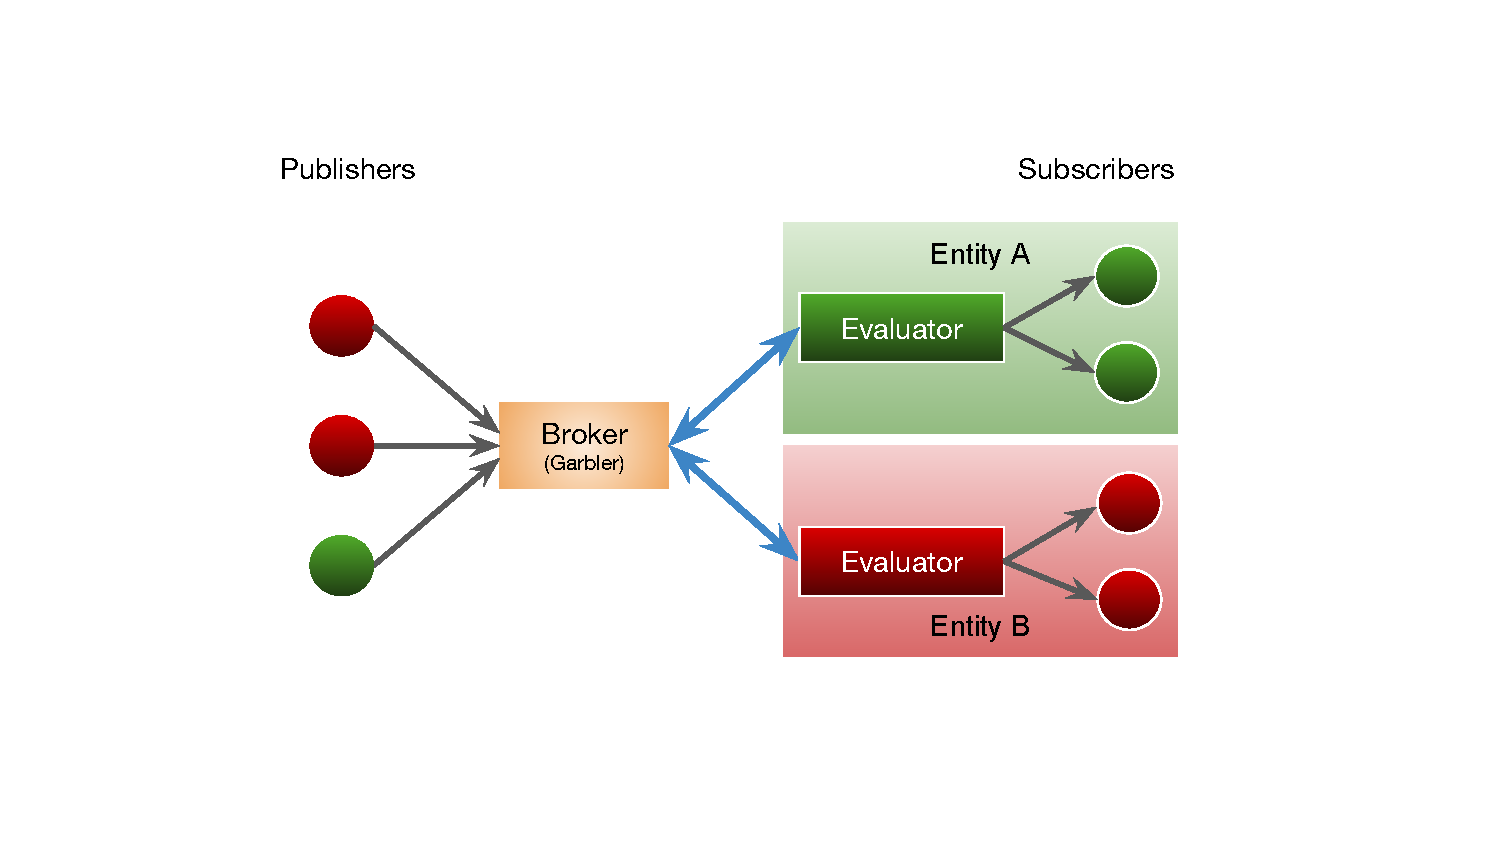
\includegraphics[width=0.95\textwidth]{figures/pps-local}
		\caption{With only \broker just like traditional topic-based publish-subscribe systems. This is suitable for large organization with several subscribers who can set up local computation.}
		\label{fig:pps-local}
	\end{subfigure}
	\begin{subfigure}{0.45\textwidth}
		\centering
		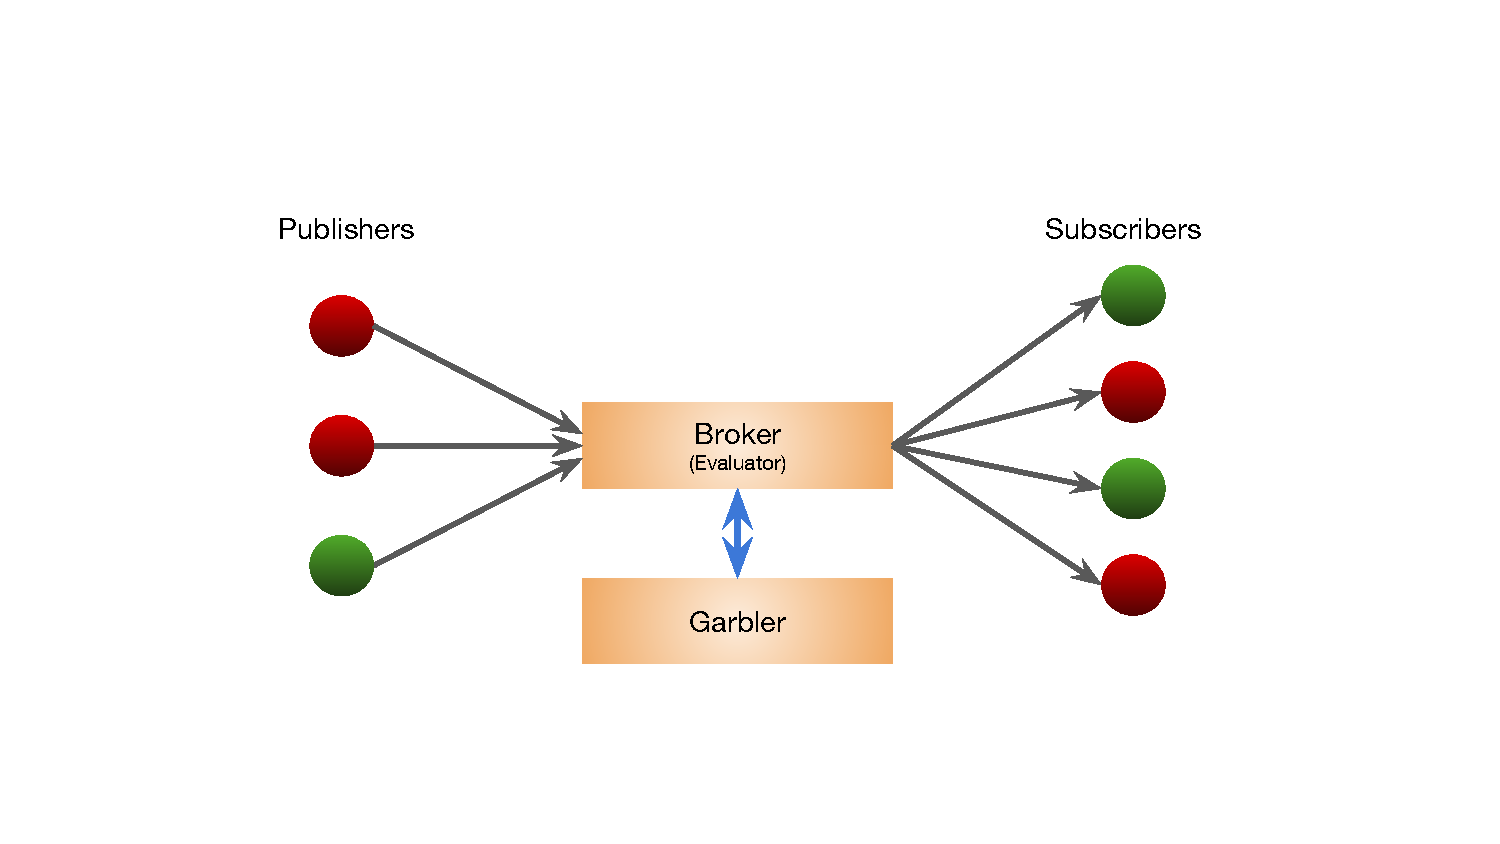
\includegraphics[width=0.95\textwidth]{figures/pps-out}
		\caption{Using a separate entity to avoid expensive processing and communication at the subscriber's end. This is suitable for mobile devices.}
		\label{fig:pps-out}
	\end{subfigure}
	\caption{Publish-Process-Subscribe System's Architecture}
	\label{fig:pps}
\end{figure}


The subscriber cannot compute it tehmselvds as they are using data from some
other entity, wihch may not want to share raw data.

\section{Related Work}
\label{sec:related}

Nikolaenko, et al., \cite{nikolaenko2013privacy} proposed a scalable
privacy-preserving system for ridge-regression combining additive homomorphic
encryption and Yao's garbled circuits.  In their setting, a single evaluator is
interested in learning ridge regression over data of a large number of data
owners without learning the individual data of data owners. Our setting and
approach is different: (\emph{a.}) we don't want to reveal output to the
evaluator, (\emph{b.}) we have multiple subscribers who want the output of
computation, (\emph{c.}) our data owners, publishers, are oblivious of
subscribers and subscribers are oblivious of publishers, (\emph{d.}) we support
arbitrary polynomial-time computations as opposed to just ridge regression, and
(\emph{e.}) we don't necessarily need a third party \garbler, as shown in
Figure~\ref{fig:pps-local} if a set of subscribers controlled by a single
entity can do a modest amount of computation. Nikolaenko, et
al.,\cite{nikolaenko2013privacy} proposed a similar system but for
privacy-preserving matrix factoring as opposed to ridge regression.

Naveed, et al., \cite{naveed2014controlled} proposed a new primitive called
controlled functional encryption inspired by functional encryption. Instead of
using the same key for computing the function over multiple ciphertexts,
controlled functional encryption requires a fresh function key for every
ciphertext. They construct an efficient controlled functional encryption scheme
for arbitrary polynomial-time computations based on Yao's garbled circuits and
CCA2 secure public key encryption. Their setting involves a data owner who
wants a client to perform only certain computations on it's data with the help
of an online key authority. Their setting is similar to our setting of
Figure~\ref{fig:pps-local}; however, in our setting publishers and subscribers
are oblivious to each other.

Fully homomorphic encryption allows arbitrary computation on encrypted data.
Gentry proposed the first fully homomorphic encryption
scheme \cite{brakerski2011fully,gentry2009fully} followed by several
improvfed schemes, e.g., Brakerski, et al., BGV scheme
\cite{brakerski2014leveled}. Dijk, et al., \cite{van2010impossibility}
showed that privacy-preserving outsourced computation on data from multiple
parties and supplying output to multiple parties, our setting, requires, in
addition to fully homomorphic encryption, access-controlled ciphertexts and
re-encryption. They reduce a scheme that computes on data from two parties
and supply the output to two parties to black box program obfuscation, which
is impossible in general \cite{barak2001possibility}.

\section{Security Definition}
\label{sec:definition}

\improvement{Explain how pub/sub works}
Before defining security, we present threat model that our definition needs to
capture.

\improvement{Explain later that publishers cannot control which subscribers can
subscribed and similary susbcriber cannot determine which publishers will be
used. Publisher either allows data for all subscribvers or noone at all; this
is how pub/sub model works. However, \broker can control which entieies can
subscribe.}

\vspace{-10pt}
\subsection{Threat Model} We assume that the adversary can \emph{maliciously}
compromise a subset of subscribers and a subset of publishers and
\emph{passively} compromise either \broker or \garbler, but not both.
Malicious subscribers and publishers can collude either with \garbler or
\broker, but not both.

\vspace{-10pt}
\subsection{Definition}

We define security for a secure publish-process-subscribe protocol in
REAL/IDEAL paradigm. Our definition captures both confidentilaity and
correctness against adversary discussed above in the threat model.\\[6pt]
\noindent\textbf{Ideal World.}
Our ideal functionality \F interacts with publishers, subscribers, \broker, and
\garbler as follows:

\begin{itemize}[leftmargin=*,itemsep=4pt,topsep=4pt]
		\item Each publisher sends a \policy to \F and each subscriber sends a
			subscription message to \F containing subscribed computation $C$. Let $S_C$
			be the set of $C$'s subscribers. 
			
%		Let $p_0, \ldots, p_{m-1}$ be the publishers whose data is required to
			%		compute $C$. 
		
		\item The honest publishers upload data to \F. The malicious publishers
			controlled by \Adv may abort (by not sending anything), sends their
			actual input, or send any arbitrary value that may depend upon their
			input, other malicious publishers' input, and auxiliary data. If a
			publisher value is not received before a time out period, \F uses a
			nullifying value for its input, e.g., $0$ for addition and $1$ for
			multiplication. 
			%We call $i$th publisher's input $x_i$; $0 \leq i < m$, $m$ being the
			%total number of publishers. 
		
		\item \garbler uploads to \F a one-time use pseudorandom mask $r$.

		\item \F determines a subset $P' \subset P$ of publishers whose data can be
			used to compute $C$. \F sends to \broker $P'$, policies of all publishers
			in $P'$, and $C$.

		\item \broker sends \F a subset $P_C \subset P'$ of publishers whose
			policies allow $C$.
			
		\item If data $\vec{x}_C$ of all publishers in $P_C$ is enough to compute
			$C$, \F sends $C(\vec{x}_C) \xor r$ and $r$ to all subscribers in $S_C$,
			otherwise \F sends empty message $\bot$ to all subscribers in $S_C$.

\end{itemize}
\vspace{6pt}
\noindent\textbf{Real World.} In real world, \F is replaced by our
protocol described in Figure~\ref{fig:baseprotocol}.\\

\begin{mdframed}[style=mydefframe]

\begin{define}
	\label{def:security}

	\textit{	A publish-process-subscribe protocol is simulation secure if for
	every adversary \Adv in the real world that maliciously corrupts a subset of
	publishers and a subset of subscribers, and only passively corrupts \broker
	and \garbler, with arbitrary collusion between malicious publishers,
	malicious subscribers, and hones-but-curious \broker and \emph{no} collusion
	between \broker and \garbler, there exists a simulator \Sim in the ideal
	world that also corrupts the same set of parties and produces an output
	identically distributed to \Adv's output in the real world.  
	}

\end{define}

\end{mdframed}

\section{Protocol}
\label{sec:protocol}

\improvement{Maliciosu \broker doesn't affect privacy, online correctness}


\begin{figure*}[h]
\begin{mdframed}[style=myframe]

%\begin{itemize}[leftmargin=*, itemsep=6pt]

\initialize
\begin{itemize}[leftmargin=*]
 
	\item Each new publisher sends \broker a \policy specifying allowed
		computations on its data.

\end{itemize}

\subscribe
\begin{itemize}[leftmargin=*]

	\item To subscribe computation $C$, subscriber sends a subscription request
		containing $C$ to \broker. If \broker allows subscriber to learn $C$'s
		output, it adds the subscriber to a list of $C$'s subscribers. 

\end{itemize}

\publish
\begin{itemize}[leftmargin=*]
		
	\item To publish $k$th value, publisher generates two pseudorandom wire
		labels, $w_0$ and $w_1$, for each bit of the value. 
		
	\item For each input bit $b$, publisher sends only $w_b$ to \broker and sends
		both $w_0$ and $w_1$ to \garbler.

\end{itemize}

\process
\begin{itemize}[leftmargin=*]

	\item \broker waits for a specified time period $t$ to receive input wire
		labels, a single label $w_b$ for a bit $b$, from a subset of publishers
		$P_C$ whose policies allow $C$. After time period $t$, \broker sends
		\garbler identifiers of publishers in $P_C$ along with identifiers of
		publishers whose data wasn't received during time period $t$ and requests
		\garbler to garble circuit for $XOR \circ C$. $XOR$ is used to mask the
		output of the circuit.

	\item \broker sends \garbler the set of $C$'s subscribers $S_C$.
		
	\item \garbler generates a garbled circuit $GC$ for the circuit $XOR \circ C$
		using both wire labels for each input bit, $w_0$ and $w_1$ for a bit $b$,
		received from publishers in set $P_C$ hard-wiring nullifying value for
		publishers whose input labels weren't received by \broker as well as any
		publishers whose labels weren't received by \garbler. \garbler generates a
		random mask $r$ and use it to mask the output $o$ of $C$, such that
		evaluating $GC$ would result in a masked output $o+r$.
		
	\item \garbler sends $r$ to all subscribers in the set $S_C$ and $GC$ to
		\broker along with identifiers for publishers for which it hard-wired
		nullifying values.

	\item For every bit $b$ of the $C$ inputs, \garbler and \broker run a
		private set intersection \emph{cardinality} (PSI-C) protocol to determine
		wire labels consistency, i.e., if \broker input label for bit $b$, $w_b$,
		is one of the two \garbler labels for bit $b$, $w_0$ and $w_1$. If PSI-C
		outputs $1$, then the labels are consistent and if it's $0$ then the labels
		are inconsistent. \garbler will use nullifying values for all inconsistent
		wire labels. 
		
	\item \broker evaluates the garbled circuit using wire labels sent by
		publishers in set $P_C$ ignoring labels for which \garbler hard-wired
		nullifying values, obtains masked output $o \xor r$, and sends $o \xor r$
		to all subscribers of computation $C$.
  
	\item Subscribers in the set $S_C$ use mask $r$ to unmask the output $o$.

\end{itemize}

\end{mdframed}
\caption{Basic Protocol}
\label{fig:basicprotocol}
\end{figure*}


\begin{figure}[h]
\begin{mdframed}[style=myframe]

%\begin{itemize}[leftmargin=*, itemsep=6pt]

\initialize
\begin{itemize}[leftmargin=*]
 
	\item Each new publisher generates and sends to \garbler a truly random seed
		$s$. This seed will be used to create wire labels without interaction.

\end{itemize}

\subscribe
\begin{itemize}[leftmargin=*]

	\item In addition to registering subscription with \broker, subscribers for a
		computation $C$ also register with \garbler. \garbler sends a truly
		random seed $s'$ for computation $C$ and send it to every subscriber who
		subscribes for $C$; generating a new seed for the first subscription for
		computation $C$.
		
\end{itemize}

\publish
\begin{itemize}[leftmargin=*]
		
	\item To publish $k$th value, publisher generates two pseudorandom wire
		labels, $w_0$ and $w_1$, using seed $s$, for each bit of the value.  $w_0$
		is $i$th and $w_1$ is $(i+1)$th numbers in pseudorandom sequence generated
		using seed $s$; $2kL \leq i < 2(k+1)L$, $L$ being the bit-length of a
		value.

	\item For each input bit $b$, publisher sends only wire label $w_b$ to
		\broker.

\end{itemize}

\process
\begin{itemize}[leftmargin=*]

	\item \garbler independently generates input wire labels using seed $s$ from
		each publisher contributing input and an output mask $r$ using seed $s'$
		for the output.

\end{itemize}

\end{mdframed}
\caption{Improved Protocol}
\label{fig:basicprotocol}
\end{figure}

\paragraph{Forward Security.}
\unsure{Do we have to generate seed and ratchet key? Can't we use the seed as a
ratchet key?}

\begin{figure}[h]
\begin{mdframed}[style=myframe]

\begin{itemize}[leftmargin=*]

		\item Generate a truly random key $K_0$.

		\item Generate, using KDF with key $K_0$, a pseudorandom seed $s_0$ and a
			pseudorandom key for the ratchet round $1$. Seed $s_0$ is used to
			generate pseudorandom strings during ratchet round $0$.

		\item At round $r$, using KDF with key $K_r$, generate a pseudorandom seed
			$s_r$ and key for ratchet round $r+1$. Seed $s_r$ is used to generate
			pseudorandom strings during ratchet round $r$.

\end{itemize}

\end{mdframed}
\caption{Forward Secure Seeds for Improved Protocol}
\label{fig:basicprotocol}
\end{figure}

\paragraph{Garbled Circuit XOR Compatibility.}


* What if one publisher doesn't send wire labels. After timeout the broker can
inform the \garbler and it will use zero for such values in the circuit.

\improvement{We can hide $C$ using universal circuits.}
\unsure{Who forms the topics? Publishers, clients, or broker?}


\improvement{Using cut and choose for malicious security}

\unsure{What is our current model? Are publishers, subscribers malicious?}

\improvement{A publisher can always input wrong data, but there is nothing that
can be done for this? May be it could be detected if it is creating a real
problem.}

\improvement{A subscribing entity can setup it's own \garbler. First we explain
with \garbler as a separate tntity and then later explain how it can be
eliminated by transfering it's functionality to subscribers. Similary, we can
transfer some functionality to publishers. Which one of them is better?}

\subsection{Security Definition}

\improvement{Explain later that publishers cannot control which subscribers can
subscribed and similary susbcriber cannot determine which publishers will be
used. Publisher either allows data for all subscribvers or noone at all; this
is how pub/sub model works. However, \broker can control which entieies can
subscribe.}

\paragraph{Ideal World.}
Our ideal functionality \F interacts with publishers, subscribers, \broker, and
\garbler as follows:

\begin{itemize}[leftmargin=*]
		\item Each publisher sends a \policy to \F and each subscriber sends a
			subscription message to \F containing subscribed computation $C$. Let $S_C$
			be the set of $C$'s subscribers. 
			
%		Let $p_0, \ldots, p_{m-1}$ be the publishers whose data is required to
			%		compute $C$. 
		
		\item The honest publishers upload data to \F. The malicious publishers
			controlled by \Adv may abort (by not sending anything), sends their
			actual input, or send any arbitrary value that may depend upon their
			input, other malicious publishers' input, and auxiliary data. If a
			publisher value is not received before a time out period, \F uses a
			nullifying value for its input, e.g., $0$ for addition and $1$ for
			multiplication. 
			%We call $i$th publisher's input $x_i$; $0 \leq i < m$, $m$ being the
			%total number of publishers. 
		
		\item \garbler uploads to \F a one-time use pseudorandom mask $r$.

		\item \F determines a subset $P' \subset P$ of publishers whose data can be
			used to compute $C$. \F sends to \broker $P'$, policies of all publishers
			in $P'$, and $C$.

		\item \broker sends \F a subset $P_C \subset P'$ of publishers whose
			policies allow $C$.
			
		\item If data $x_C$ of all publishers in $P_C$ is enough to compute $C$, \F
			sends $C(\vec{x_C}) \xor r$ and $r$ to all subscribers in $S_C$,
			otherwise \F sends empty message $\bot$ to all subscribers in $S_C$. 

\end{itemize}

\paragraph{Real World.} In real world, \F is replaced by our protocol~\ref{}.

\noindent\textbf{Simulator.}
%\improvement{Inconsistent wire labels}
%
%The intereseting case is when publishers are corrupt and \broker and \garbler are hones-but-curious.
%
%\Adv sends \Sim inputs of all malicious publishers. \Sim uses zero inputs for
%honest publishers. \Sim generates wire labels for all inputs 
%
%\Sim sends all inputs and output mask $r$ to \F and learns
%$\F(M \circ C, \vec{x})$, whre $M$ is an XOR masking function. \Sim sends $\F(M
%\circ C, \vec{x})$ to $\Sim_{GC}$ and obtains a fake garbled $GC_{fake}$. \Sim
%generates a single random wire label for each wire of the circuit. \Sim sends
%$GC_{fake}$ and wire labels to \Adv.  $\Sim_{GC}$ is computationally
%indistinguishable from the garbled circuit generated in the real execution, as
%garbled circuit distribution doesn't depend upon on the input values. The
%pseudorandom wire labels are also computational indistinguishable from actual
%wire labels.
%
%This proof implies both privacy and correctness as distribution in both the
%real and ideal world have a negligible difference. 
%
%
%\Sim generates random wire labels for all wires of the circuit $M \circ C$. 
%
%\Sim receives from \F a handle $h_C$ and the number of publishers $|P_C|$ whose
%policy allow $C$. \Sim 
The interesting case is when up to all-but-one publishers are malicious and are
colluding with honest-but-curious \broker. A malicous \broker affects
correctness but not privacy. A malicious subscriber only receives output; it
can only reveal its own output, which is possible in ideal execution as well.

\Sim receives from \F the number of publishers $|P_C|$ whose policy allow
computing $C$ on their data. \Sim creates $2l|P_C|$ random wire labels $(r_0^0,
r_0^1), \ldots, (r_{2l|P_C|-1}^0 ,r_{2l|P_C|-1}^1)$; $l$ being the bit-length
of a publisher's input. We use garbled circuit simulator $\Sim_{GC}$ as a
blackbox; $\Sim_{GC}$ is the simulator of the projective prv.sim secure
garbling scheme with circuit $M \circ C$ being the side information as
described in~\cite{}. 

\Sim receives from \F $\F(M \circ C, \vec{x_C})$, where $M$ is an XOR masking
function. \Sim sends $\F(M \circ C, \vec{x_C})$ to $\Sim_{GC}$ and obtains a
fake garbled $GC_{fake}$. \Sim generates a random string $o_r$ of the same
length as output. \Sim sends $(GC_{fake}, r_0^0, \ldots, r_{2l|P_C|-1}^0, o_r)$
to \Adv. As garbled circuits distribution is indepedent of the input wire
labels, $GC_{fake}$ is computationally indistinguishable from the $GC$ in the
real execution. The random output $o_r$ in ideal execution is indistinguishable
from $o+r$ in the real execution.

In the ideal world, \Sim creates a fake garbled circuit $GC_{fake}$ that
doesn't use wire labels $(r_0^0, r_0^1), \ldots, (r_{2l|P_C|-1}^0
,r_{2l|P_C|-1}^1)$ for garbling. Otherwise, \Adv could use $r_0^0, \ldots,
r_{2l|P_C|-1}^0$ labels to evaluate the circuit on $0^{l|P_C|}$, which would
allow adversary to distinguish between real and ideal executions.

A malicious publisher can choose arbitrary wire labels in the real execution;
however, as long as the labels used in garbling are consistent with the labels
used for evluation, the honest subscriber output will be indistinguishable in
real and ideal executions. Our protocol ensures consistent wire labels. 

Our threat model allows for publishers and subscribers to collude aribitrailly.
\broker and \garbler are semihonest.


%\Sim generates a single random wire label for each
%wire of the circuit. \Sim sends $GC_{fake}$ and wire labels to \Adv.
%$\Sim_{GC}$ is computationally indistinguishable from the garbled circuit
%generated in the real execution, as garbled circuit distribution doesn't depend
%upon on the input values. The pseudorandom wire labels are also computational
%indistinguishable from actual wire labels.
%
%
%We ensure such consistency
%using private set intersection cardinarlity between  
%
%
%
%
%In the real execution, a
%malicious publisher can send inconsistent wire labels to \broker and \garbler;
%which will result in \broker being unable to evalute the garbled circuit. \broker
%and \garbler use private set intersection cardinality to ensure that \broker and \garbler labels are consistent. 
%
%A malicious publisher may send
%non-random wire labels or inconsistent wire labels. To make the wire labels
%consistent, in the real execution, \broker and \garbler use private set
%intersection cardinality to figure out if \broker has a consistent label. As
%long as this property holds, the value of the labels doesn't affect the output
%of the honest parties. 
%
%
%A malicious publisher may not
%send a random wire label in the real execution.


\section{System}
\label{sec:system}

Our protocol implementation works on top of the IoT \MQTT{} protocol, which
allows exchanging messages in a publisher-subscriber model arbitrated by a
\broker.  In order to set up the ratchet keys, both Subscribers and Publishers
need a private communication channel with the \garbler.  In order to embed
this communication into the MQTT protocol each client (either Publisher or
Subscriber) will have a device-specific topic that will allow two-way
authenticated communication between each client and the \broker.  The \broker
will forward the messages from this channel to the \garbler so that clients
can establish a ratchet key with the \garbler.  This design choice helps us
maintain the \MQTT{} semantics on the clients, since they only exchange
messages with a single \broker at the \MQTT{} level.

Although \MQTT{} can be used on top of TLS to provide secrecy, authenticity and
forward-secrecy; when clients obtain the ratchet keys from the \garbler
the communication is forwarded by the \broker at the application layer, so we
need to protect it to maintain secrecy, authenticity and forward-secrecy
against the \broker.  For this reason we choose to add authentication in the
\MQTT{} messages by means of public key signature and we use a key exchange
protocol to share secrets between Clients and the \garbler.  In the case of
Publishers, this authenticated key exchange is used to derive the Publisher'
ratchet key.  In the case of Subscribers, for every function subscription, a
key exchange is performed to derive a key to encrypt the function ratchet key
sent from the \garbler to the Subscriber.

\noindent\textbf{Ratchet keys}.  The use of shared ratchet keys between
Publishers and the \garbler, and between the Subscribers and the \garbler
allows us to maintain forward secrecy at the published value level and at the
function output level at a very low cost.  With this we achieve the property
that if an attacker gets hold of the secret keys from any participantin the
protocol, this attacker will not be able to decrypt past values even if they
have recorded all previous communications.  Ratchet keys work by advancing a
secret key every at round (by means of using the using the preimage-resistance
of a cryptographic hash function).  At any round, a seed can be derived from a
ratchet key to be used to generate pseudorandom byte strings.  The idea of
using ratchet keys to achieve forward secrecy has been popularized by the
Signal messaging protocol (already analyzed by the security research
community~\cite{signal1}~\cite{signal2}), from which we take inspiration.

This design achieves the desired cryptographic properties of TLS for selected
parts of the messages underlying the \MQTT{} communication, allowing the \broker
to be aware of the operation without being able to reveal or tamper with any
ratchet key.

\noindent\textbf{Seed syncrhonization}. To maintain syncrhonization of the
ratchet keys between the clients and the \garbler, when sending values the
Publisher adds the round of the ratchet key used to derive the seeds used to
generate the labels in the message.  When the \broker requests the garbling of
the circuit to the \garbler, it also specifies the rounds of the values it will
use, so that the \garbler can advance the Publisher ratchet key accordingly to
derive the same seed and generate matching labels.  Similarly, the \garbler
tells the \broker the function ratchet key round used to generate the mask, so
that the \broker can forward this information to the Subscribers which in turn
advance their stored ratchet keys to derive a matching mask.

During the Publisher setup phase, not only its ratchet key will be established
but also the \broker will register a special publishing topic that the Publisher
will use to submit its encrypted values.  Every time the \broker evaluates a
garbled circuit using Publishers encrypted values as inputs, it will publish
the masked result to the relevant function topic so that the interested
Subscribers can receive it after having subscribed to that function topic.

The \MQTT{} messages for our protocol are encoded in JSON, with all the binary
data encoded in base64.  A possible improvement in performance and bandwidth
usage would consist on replacing this encoding for a binary one such as
Protocol Buffers.

The block cipher behind the garbled circuit in our implementation is AES-128
(both blocks and keys are 128 bits).  In particular, the block size has a
direct relation to the size of the garbled circuit (as every non-XOR gate
requires a fixed number of cipher blocks) as well as the required bandwidth
between Publishers and the \broker, and between Subscribers and the \broker.  In
particular, for every secret bit transferred from or to a client (which will
either be an input bit or an output bit of the garbled circuit) will be
expanded to 128 bits.

\subsection{Extending \libgarble.}

\libgarble{}~\cite{libgarble} is a garbling library written in C based on
\emph{JustGarble}~\cite{justgarble} that is in current development.  It extends
\emph{JustGarble} by adding two different size optimizations in the garbled
circuit: Half-gates (which combines the free-XOR optimization with AND gates
that only require two ciphertexts) and Privacy-free garbling (which achieves
the free-XOR optimization with AND gates that only require one ciphertext at
the cost of losing privacy and only guaranteeing authenticity).  Apart from
restructuring the code to make it more concise, it also offers a better API
than \emph{JustGarble} to build circuits.

Nevertheless, \libgarble{} being in current development lacks some
functionality which we had to add in order to build circuits and garble them
according to our needs.  On the garbling side, we implemented the NOT gate
(expressed as the XOR of the input with 1 to take advantage of the free-XOR
optimization) and the OR gate.  Our implementation doesn't use the half-gates
optimization due to the fact for this mode of operation, \libgarble{} in its
current design only reserves two ciphertext per gate, not allowing the
implementation of OR gates in a straight-forward manner.

We added some arithmetic blocks to be used when building circuits in order to
allow a wide variety of functions to be described: \textbf{signed fixed point
multiplication}, \textbf{signed fixed point division} and \textbf{signed
min/max}.

The motivation to operate with fixed point numbers was to be able apply
arbitrary functions based on arithmetic operations without the constraint of
having just integer values.  Even though it would be easy to scale input values
to be integers maintaining the desired precision, it's common in several
algorithms used in our applications to have intermediate values with decimals
that are significant.

A similar reasoning goes for supporting signed numbers.  We use the common
two's complement to represent such numbers, which work straightforward for
addition and integer multiplication but require special changes for fixed point
multiplication, division and min/max.

Whereas expanding \textbf{multiplication} and \textbf{min/max} to support
signed fixed point numbers was not hard (for multiplication we need to fix the
scaling of the result and for min/max we need to figure out the signedness of
the inputs), implementing \textbf{division} becomes a challenge.  Most of the
fast division algorithms are not fit for combinational circuits, which is a
constraint for the garbled circuits, because they assume circuit loops which we
will need to unroll, among other optimizations.  For this reason we implemented
the simplest non-optimized division algorithm: division by repeated subtraction
with a fixed number of iterations (assuming the worst case).

\subsection{High level language to build circuits.}

While \libgarble{} exposes the functions needed to build circuits corresponding
to the functions we are interested in, the process becomes cumbersome and error
prone.  To facilitate building circuits from functions we have implemented an
interpreter for a functional programming language inspired in Scheme, a dialect
of Lisp.  This choice was motivated both by the simplicity of parsing a
Lisp-like language as well as the similarity between the descriptive nature of
functional languages with combinational circuits, which helps reasoning about
how the circuit is built.  Moreover, the availability of high-order functions
in the language (functions that take functions as arguments and/or return
functions as a result) allows us to express circuits that combine building
blocks very concisely.

The interpreter is written in golang in just 470 lines of code.

Other solutions to express garbled circuits in higher level languages than the
underlying gates themselves have been proposed: namely \OblivC{}~\cite{oblivc}.
\OblivC{} allows the developer to embed the secure computation part of a
protocol in C code with a GCC wrapper that takes care of the compilation, the
circuit building and the integration in a distributed program.  We don't
require this embedding in our protocol because the secure function is directly
described independently.

\noindent
\begin{minipage}{\linewidth}
\lstinputlisting[
caption={Definition of the \emph{fold} high order function with an example of
its usage with \emph{min2} to define a new function.}]
{listings/prelude.lsp}
\end{minipage}

Where the only \libgarble{} building block is \texttt{min2}, which takes two
signed integers and returns the smaller one.

\texttt{fold} is a high order function that recursively traverses a list
\texttt{l} combining its elements with a function \texttt{f} to build up a
return value.

\noindent
\begin{minipage}{\linewidth}
\lstinputlisting[
caption={Example of a function over Publishers' values.}]
{listings/min-example.lsp}
\end{minipage}

From this function definition the interpreter is capable of constructing the
circuit that evaluates the function as well as storing the list of publisher
values required to evaluate it.

Four our implementation we decided to use the same representation for all
numerical values: two's complement fixed point 32 bit numbers, with 26 bits for
the integer part and 8 bits for the decimal part.

\subsection{\broker and \garbler.}

The \broker and the \garbler have been written in the Go programming
language.  The choice of go was motivated on one hand due to the provided
built-in concurrency facilities such as \emph{goroutines} (light-weight
threads) and \emph{channels} (a primitive to send messages between
\emph{goroutines}), which are very appropriate for the networking server nature
of both entities.  On the other hand, this language offers the good performance
of a compiled language with the benefits of memory safety (which is very
welcomed when dealing with dynamic data structures).

The communication between the \broker and \garbler (to request the garbling
of a circuit for Publishers inputs at some particular rounds) happens over a
TCP RPC synchronously.

The \broker requires a regular \MQTT{} \broker server which we take from an
open source implementation~\cite{mqttgo}.  We have modified it so that any
received message whose topic starts with a name space reserved for our
protocol, will be handled according to the protocol description instead of
being forwarded to the subscribers of that topic.

The \broker and \garbler are required to maintain replicated data structures
to store information of every Publisher, Subscriber and function.  Our design
makes this requirement easy because all setup messages between clients and
\garbler are forwarded by the \broker, allowing the later one to register the
non-secret details of the setup.

The \garbler is in charge of maintaining Publishers ratchet keys in sync
with Publishers, and Function ratchet keys in sync with Subscribers interested
in that function.  The \garbler also garbles circuits on demand for the
\broker.

The \broker is in charge of storing Publishers encrypted values with their
corresponding publisher ratchet key round, and of requesting the garbling of
circuits to the \garbler (for those particular Publishers values rounds) to
evaluate the garbled circuit and send the result to the subscribed Subscribers.

\subsection{Publisher and Subscriber.}

The Publisher has been written in C in order to minimize its memory footprint
as well as its resource consumption, considering that the code may be running
in a resource-constraint IoT device.  For the \MQTT{} part of the Publisher we
have used the Eclipse Paho client library~\cite{paho}.

On the other hand, the Subscriber has been written in golang, assuming that it
will be running on a more powerful device.  The \MQTT{} library used by the
Subscriber is the same we used in the \broker\~cite{mqttgo}, which also provides
client functionality.

Publishers and Subscribers follow a state machine to initialize themselves
(i.e.\ for Publishers to obtain a Publisher ratchet key, for Subscribers to
obtain the Function ratchet key of all desired functions).  The initialization
to establish the ratchet keys happens through a message exchange with the
\broker and \garbler via \MQTT{} messages published and received at a unique
per-device specific topic.  The device specific topic is formed using the
Client's (Subscriber or Publisher) public key.

\subsection{Identity Gates for FreeXOR Compatibility.}

The free XOR optimization in garbled circuits require that for every wire, the
XOR of the label for bit 0 and bit 1 be a unique secret constant \emph{delta}
value.  Since input values are generated by independent Publishers using their
own seed, it's not easy to achieve this pattern without adding complexity to
the system.  For this reason, the \garbler will generate one \emph{identity}
gate per input wire that will allow transforming the inputs sent by Publishers
to garbled circuit inputs that follow the \emph{delta} pattern.

The implementation of these identity gates has been written in Go and is
integrated in the \broker and \garbler.  Because it's not written in C, like
the rest of the circuit garbling and garbled circuit evaluation, we consider
this step not to be optimized for speed.  Nevertheless, its computation
overhead should be small and linear in the number of the circuit function
inputs.

% OTHER STUFF

\subsection{Cryptographic choices}

For all the cryptographic operations we have used the \emph{libsodium} C
library~\cite{libsodium} which is a fork of NaCl~\cite{nacl}.  A particular
feature of this library is that it offers basic cryptographic primitives with
secure design choices for the underlying construction, algorithms and
parameters.  This provides a high level of usability and removes the
possibility of some error-prone choices.

In particular, the library makes the following choices for the primitives we use.

\begin{itemize}
  \item \textbf{Key Derivation Function}: \emph{BLAKE2B} is used for the
    underlying hash function.
  \item \textbf{Public key signatures}: \emph{Ed25519} elliptic curves are used.
  \item \textbf{Key Exchange}: Elliptic curve Diffie-Hellman with the
    \emph{Curve25519} curve (that is, \emph{X25519}) is used to obtain a shared
    secret, from which cryptographically secure keys are derived by applying
    the \emph{BLAKE2B-512} hash function.
  \item \textbf{Encryption}: The \emph{ChaCha20} stream cipher is used for
    encryption with \emph{Poly1305} MAC to provide authenticity.
  \item \textbf{CPRNG}: Uses the \emph{ChaCha20} stream cipher.
\end{itemize}

Even though \emph{libsodium} allows us to use \emph{AES} for encryption, we
choose to stick with \emph{ChaCha20} because it is faster in software-only
implementations (which is the only option available in many IoT devices) and
because it is not sensitive to cache-collision timing attacks by design.

The construction \emph{ChaCha20-Poly1305} has also been proposed as a standard
choice of ciphersuit in the upcoming TLS version 1.3, which gives us further
confidence in the decision to use it in our protocol.

\section{Evaluation}
\label{sec:evaluation}

\subsection{Setup}

We have evaluated our implementation in an environment consisting on two
computers located in the same Gigabit Ethernet network.  We run the \broker,
\garbler and one Subscriber on the first computer, and all the Publishers in
the second computer.  We perform all the analysis on the performance of several
operations in the \broker and \garbler, which run together in a computer
running Arch Linux (kernel 4.8.17-grsec) with an Intel Core i7-6600U CPU with
16GB of RAM.  In order to isolate the performance influence of the \broker and
the \garbler, we have serialized the garbling and evaluation of the garbled
circuit operations (forbidding evaluation operations while the \garbler is
garbling), mimicking the situation in which the \broker and \garbler are run on
different servers.  We also forbid concurrent garbling operations and
concurrent evaluation operations to avoid high fluctuations in the measures.

Since the \broker and the \garbler are running on the same computer, we won't
observe the delay introduced by transferring the garbled circuit over a
physical network.  For this reason we obtain an estimation of the time required
to send the garbled circuit by simulating a transmission over a Gigabit
bandwidth network.  Since we know the size of the garbled circuit, we can
easily compute the time required to transfer it over a Gigabit connection and
add that delay to the measured time.

Our current implementation doesn't support the Private Set Intersection between
\broker and \garbler used to guarantee that the labels sent by the Publishers
are valid for the garbled circuit.  In order to evaluate this step of the
protocol we have run simulations of an implementation of the Private Set
Intersection based on Oblivious Transfer extension~\cite{Pinkas0Z14}, using the
number of labels corresponding to 32 bit values.

In all our measured times, sending includes the marshaling and unmarshaling of
the garbled circuit and associated data structures necessary for transmitting
it from the \garbler to the \broker via RPC.

\vspace{-10pt}
\subsection{Microbenchmarks}

\begin{figure*}[ht]
    \centering
    \begin{subfigure}[b]{0.32\textwidth}
        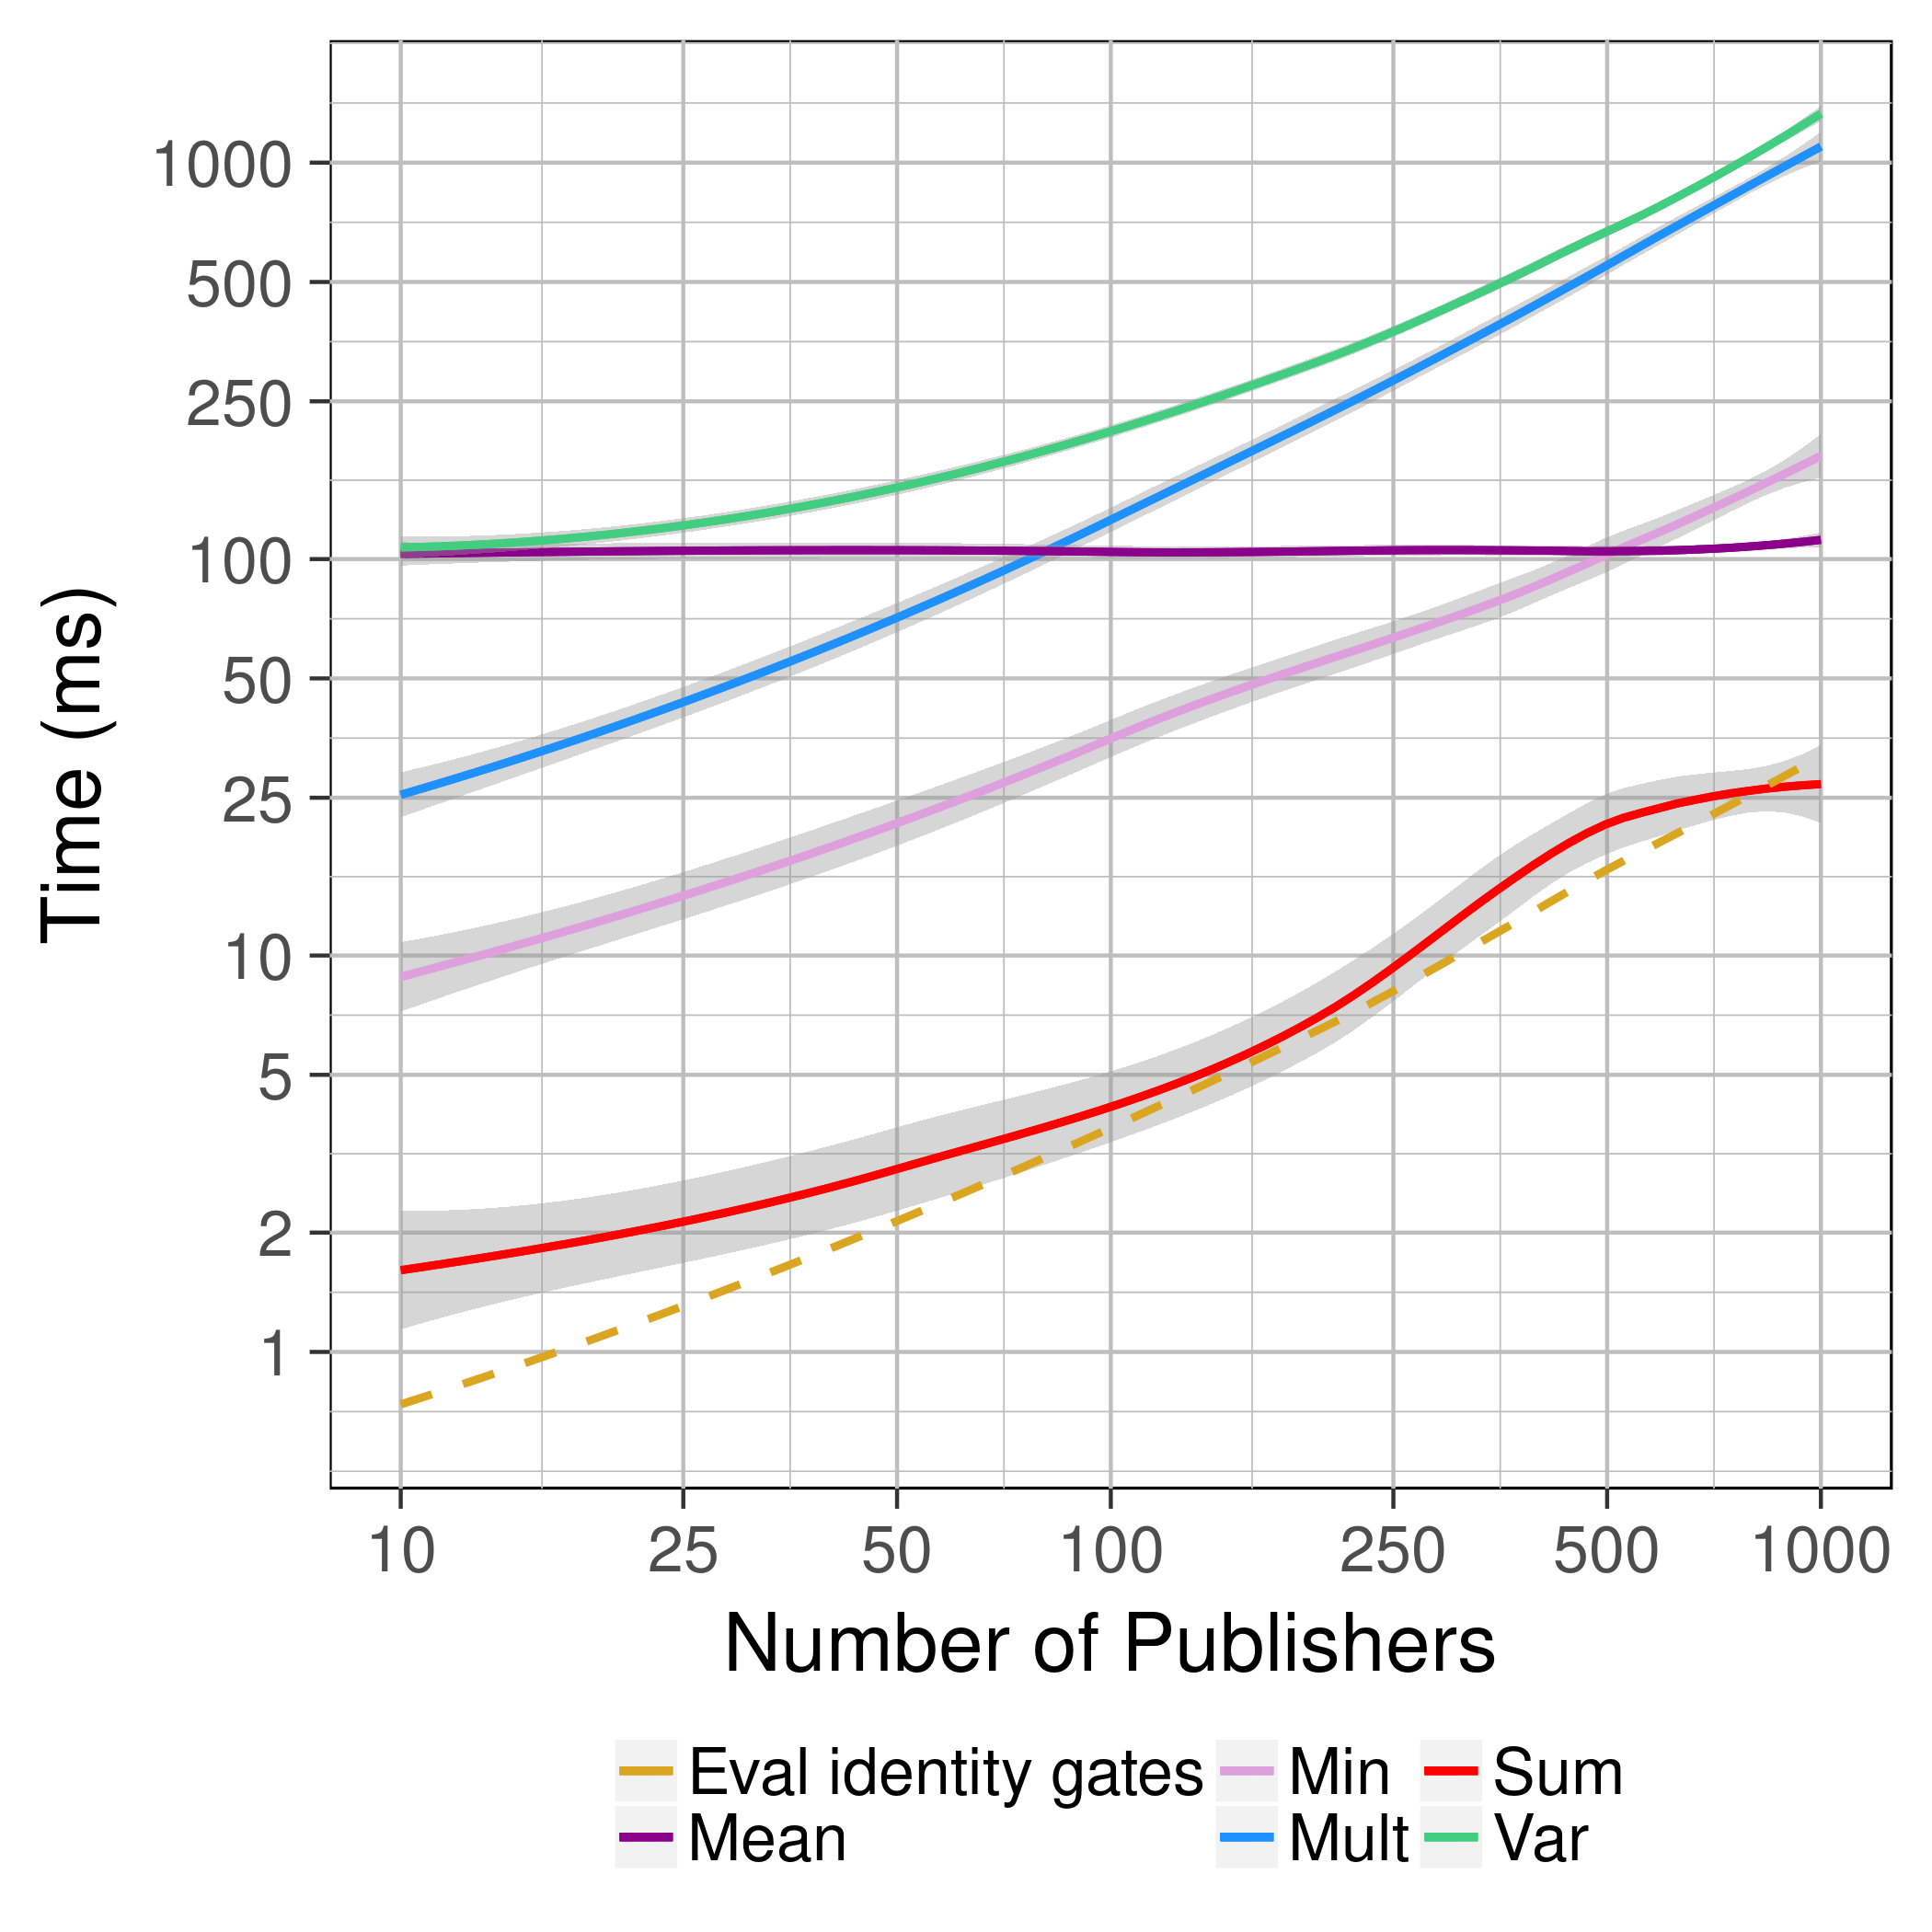
\includegraphics[width=\textwidth]{plots/garble_loglog.png}
        \caption{Garble}
        \label{fig:micro-garble-time}
    \end{subfigure}
    ~ %add desired spacing between images, e. g. ~, \quad, \qquad, \hfill etc.
    \begin{subfigure}[b]{0.32\textwidth}
        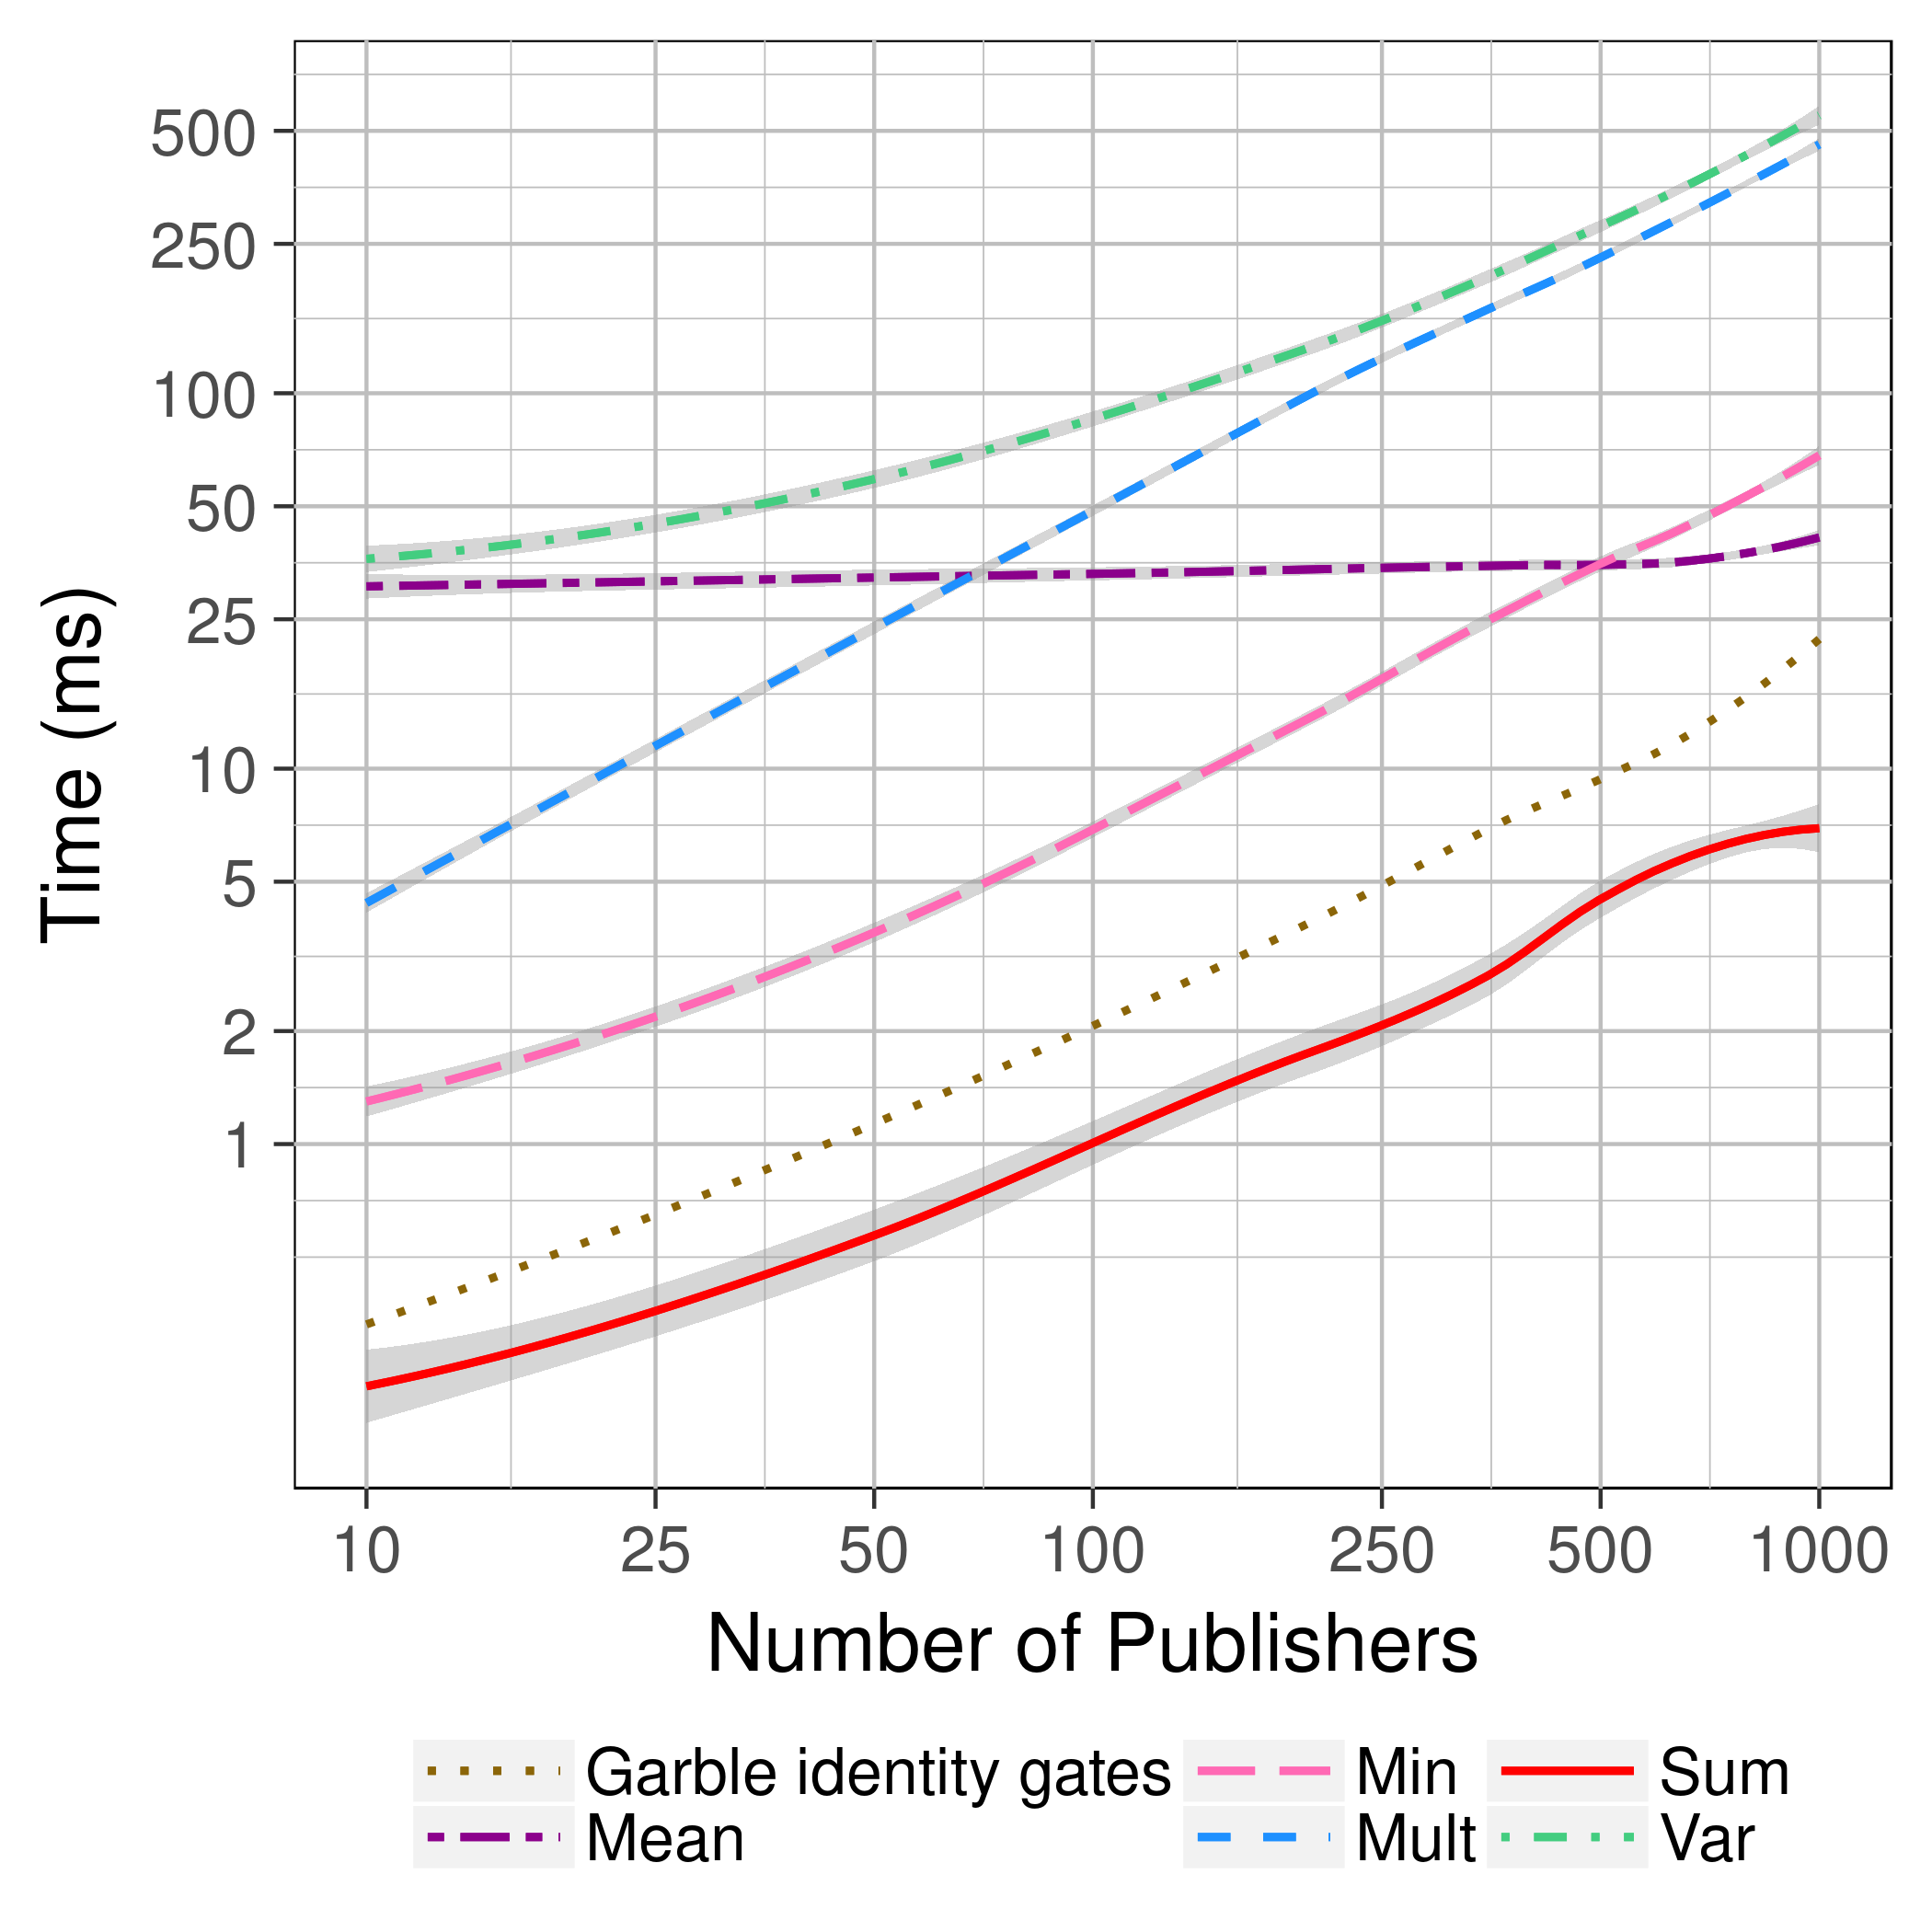
\includegraphics[width=\textwidth]{plots/eval_loglog.png}
        \caption{Evaluate}
        \label{fig:micro-eval-time}
    \end{subfigure}
    ~ %add desired spacing between images, e. g. ~, \quad, \qquad, \hfill etc.
    \begin{subfigure}[b]{0.32\textwidth}
        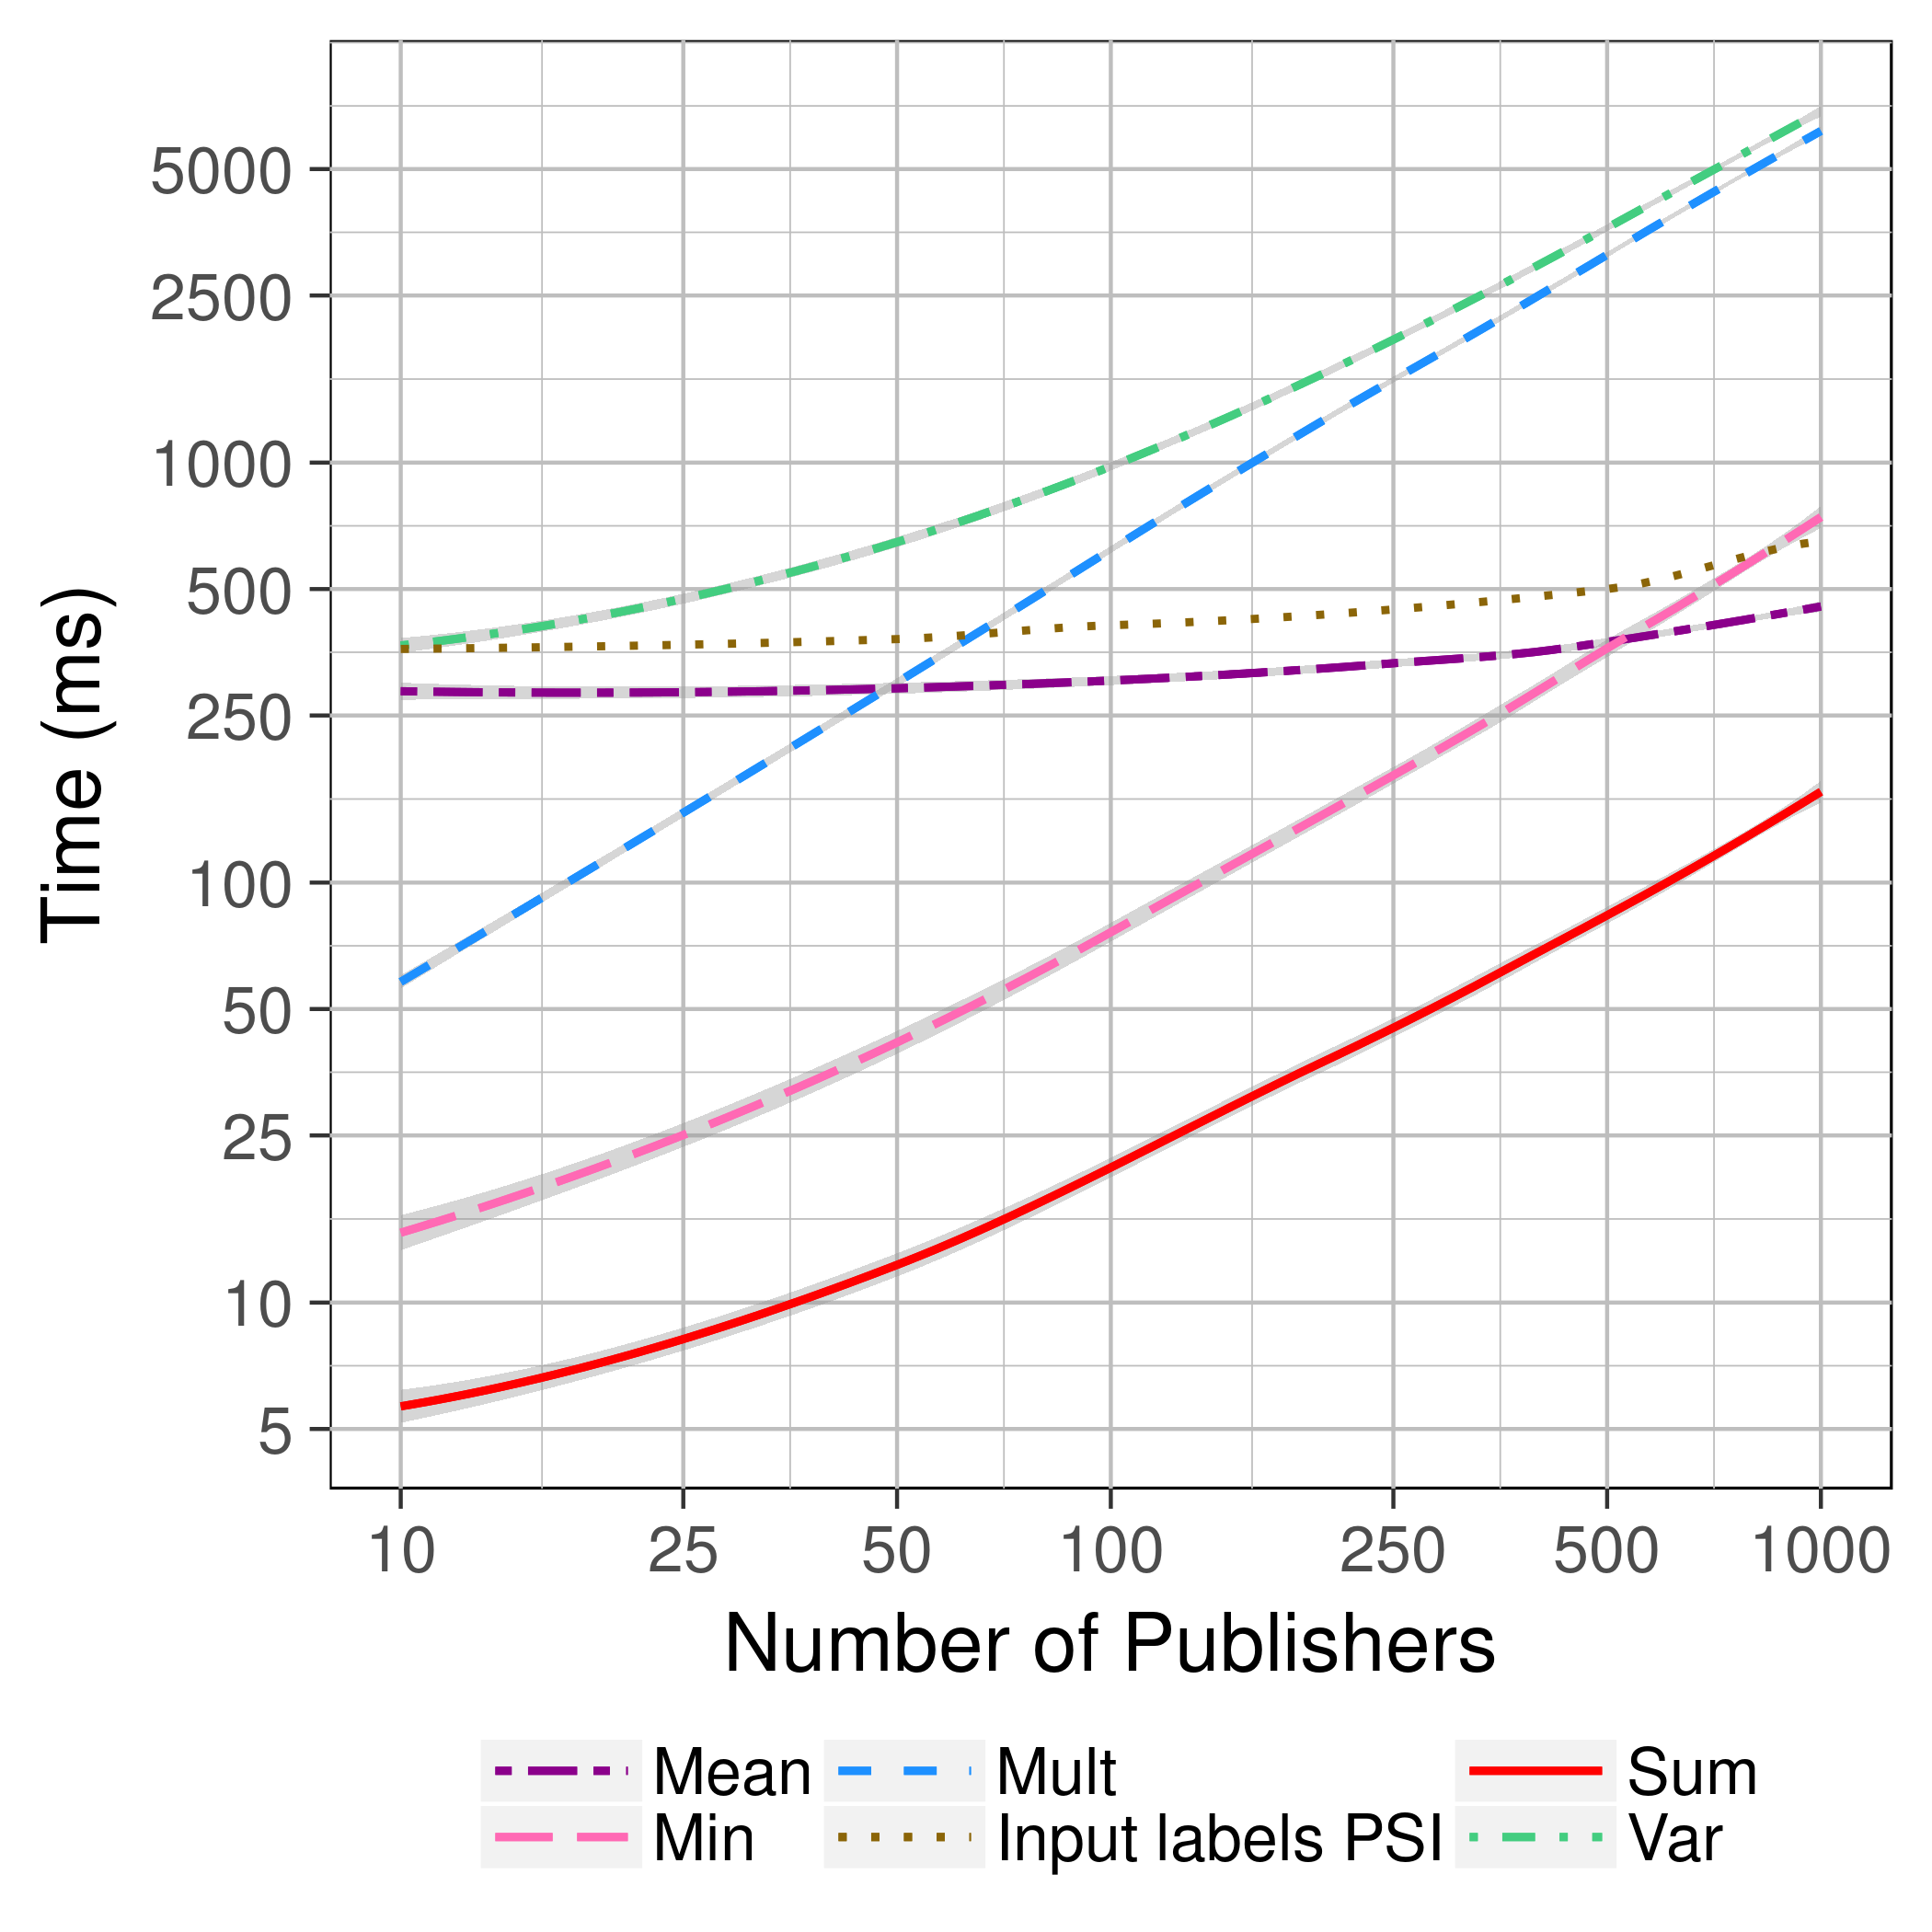
\includegraphics[width=\textwidth]{plots/send_loglog.png}
        \caption{Send}
        \label{fig:micro-send-time}
    \end{subfigure}
    \caption{Mean time required for garbling, evaluating and sending the
      garbled circuit to the \broker for each function in the microbenchmark.
      Results obtained from the mean of 5 repetitions for each configuration,
      with the confidence interval of 95\% shown in gray.}
    \label{fig:micro-times}
\end{figure*}

We have selected 5 numerical operations of varying complexity (\emph{summation,
multiplication, mean, variance, minimum/maximum}) to evaluate the cost of the
different parts of our implementation.  We securely evaluate these functions
over the values (encoded as 32 bit fixed point numbers) received from a
variable number of Publishers.

In figure~\ref{fig:micro-times} we show the timing results for the most
relevant steps of the secure computation happening between the \broker and the
\garbler of the 5 numerical operations for varying number of Publishers from 10
to 1000.  In particular, since we are encoding the Publishers values with 32
bits, the number of input wires will be the number of Publishers times 32.  We
would expect the evaluated functions to scale linearly in the three analyzed
steps of the protocol.  Whereas the \emph{multiplication} shows the more clear
linear scaling, other operations show a transitive state tending to linear,
with the most extreme case happening on the \emph{mean}.  We attribute this
later result to the fixed cost of the final division in the mean, which becomes
the dominant overhead of the circuit until the number of Pulbishers start
reaching the 1000.  On the other hand, the \emph{summation} is the most
lightweight function, and doesn't show yet a stabilizing linear trend for the
number of Publishers used in the experiment.  Accompanying the garble
(figure~\ref{fig:micro-garble-time}) and the evaluate
(figure~\ref{fig:micro-eval-time}) we show the time it took to garble and
evaluate the input identity gates.  We have also decoupled the time spent
following the Private Set Intersection between the \broker and \garbler from
the sending time, and we show it in figure~\ref{fig:micro-send-time}.

We can see that the time spent dealing with the identity gates (encrypting and
decrypting the inputs) makes a significant influence in the faster functions,
being comparable in magnitude to the evaluation and garbling time of the
\emph{summation} (the input decryption time is even higher than the garbled
circuit evaluation time for \emph{summation}).  We attribute this behavior to
the fact that this part of the protocol is implemented in Go instead of C like
the garbling and evaluation.

We can also see how the time spent on the Private Set Intersection protocol is
higher than the time required for sending in the case of the \emph{Mean},
\emph{Min} and \emph{summation}, although it seems that it will scale better
than the later two functions when the number of Publishers well passes the
thousands.

\begin{figure}
  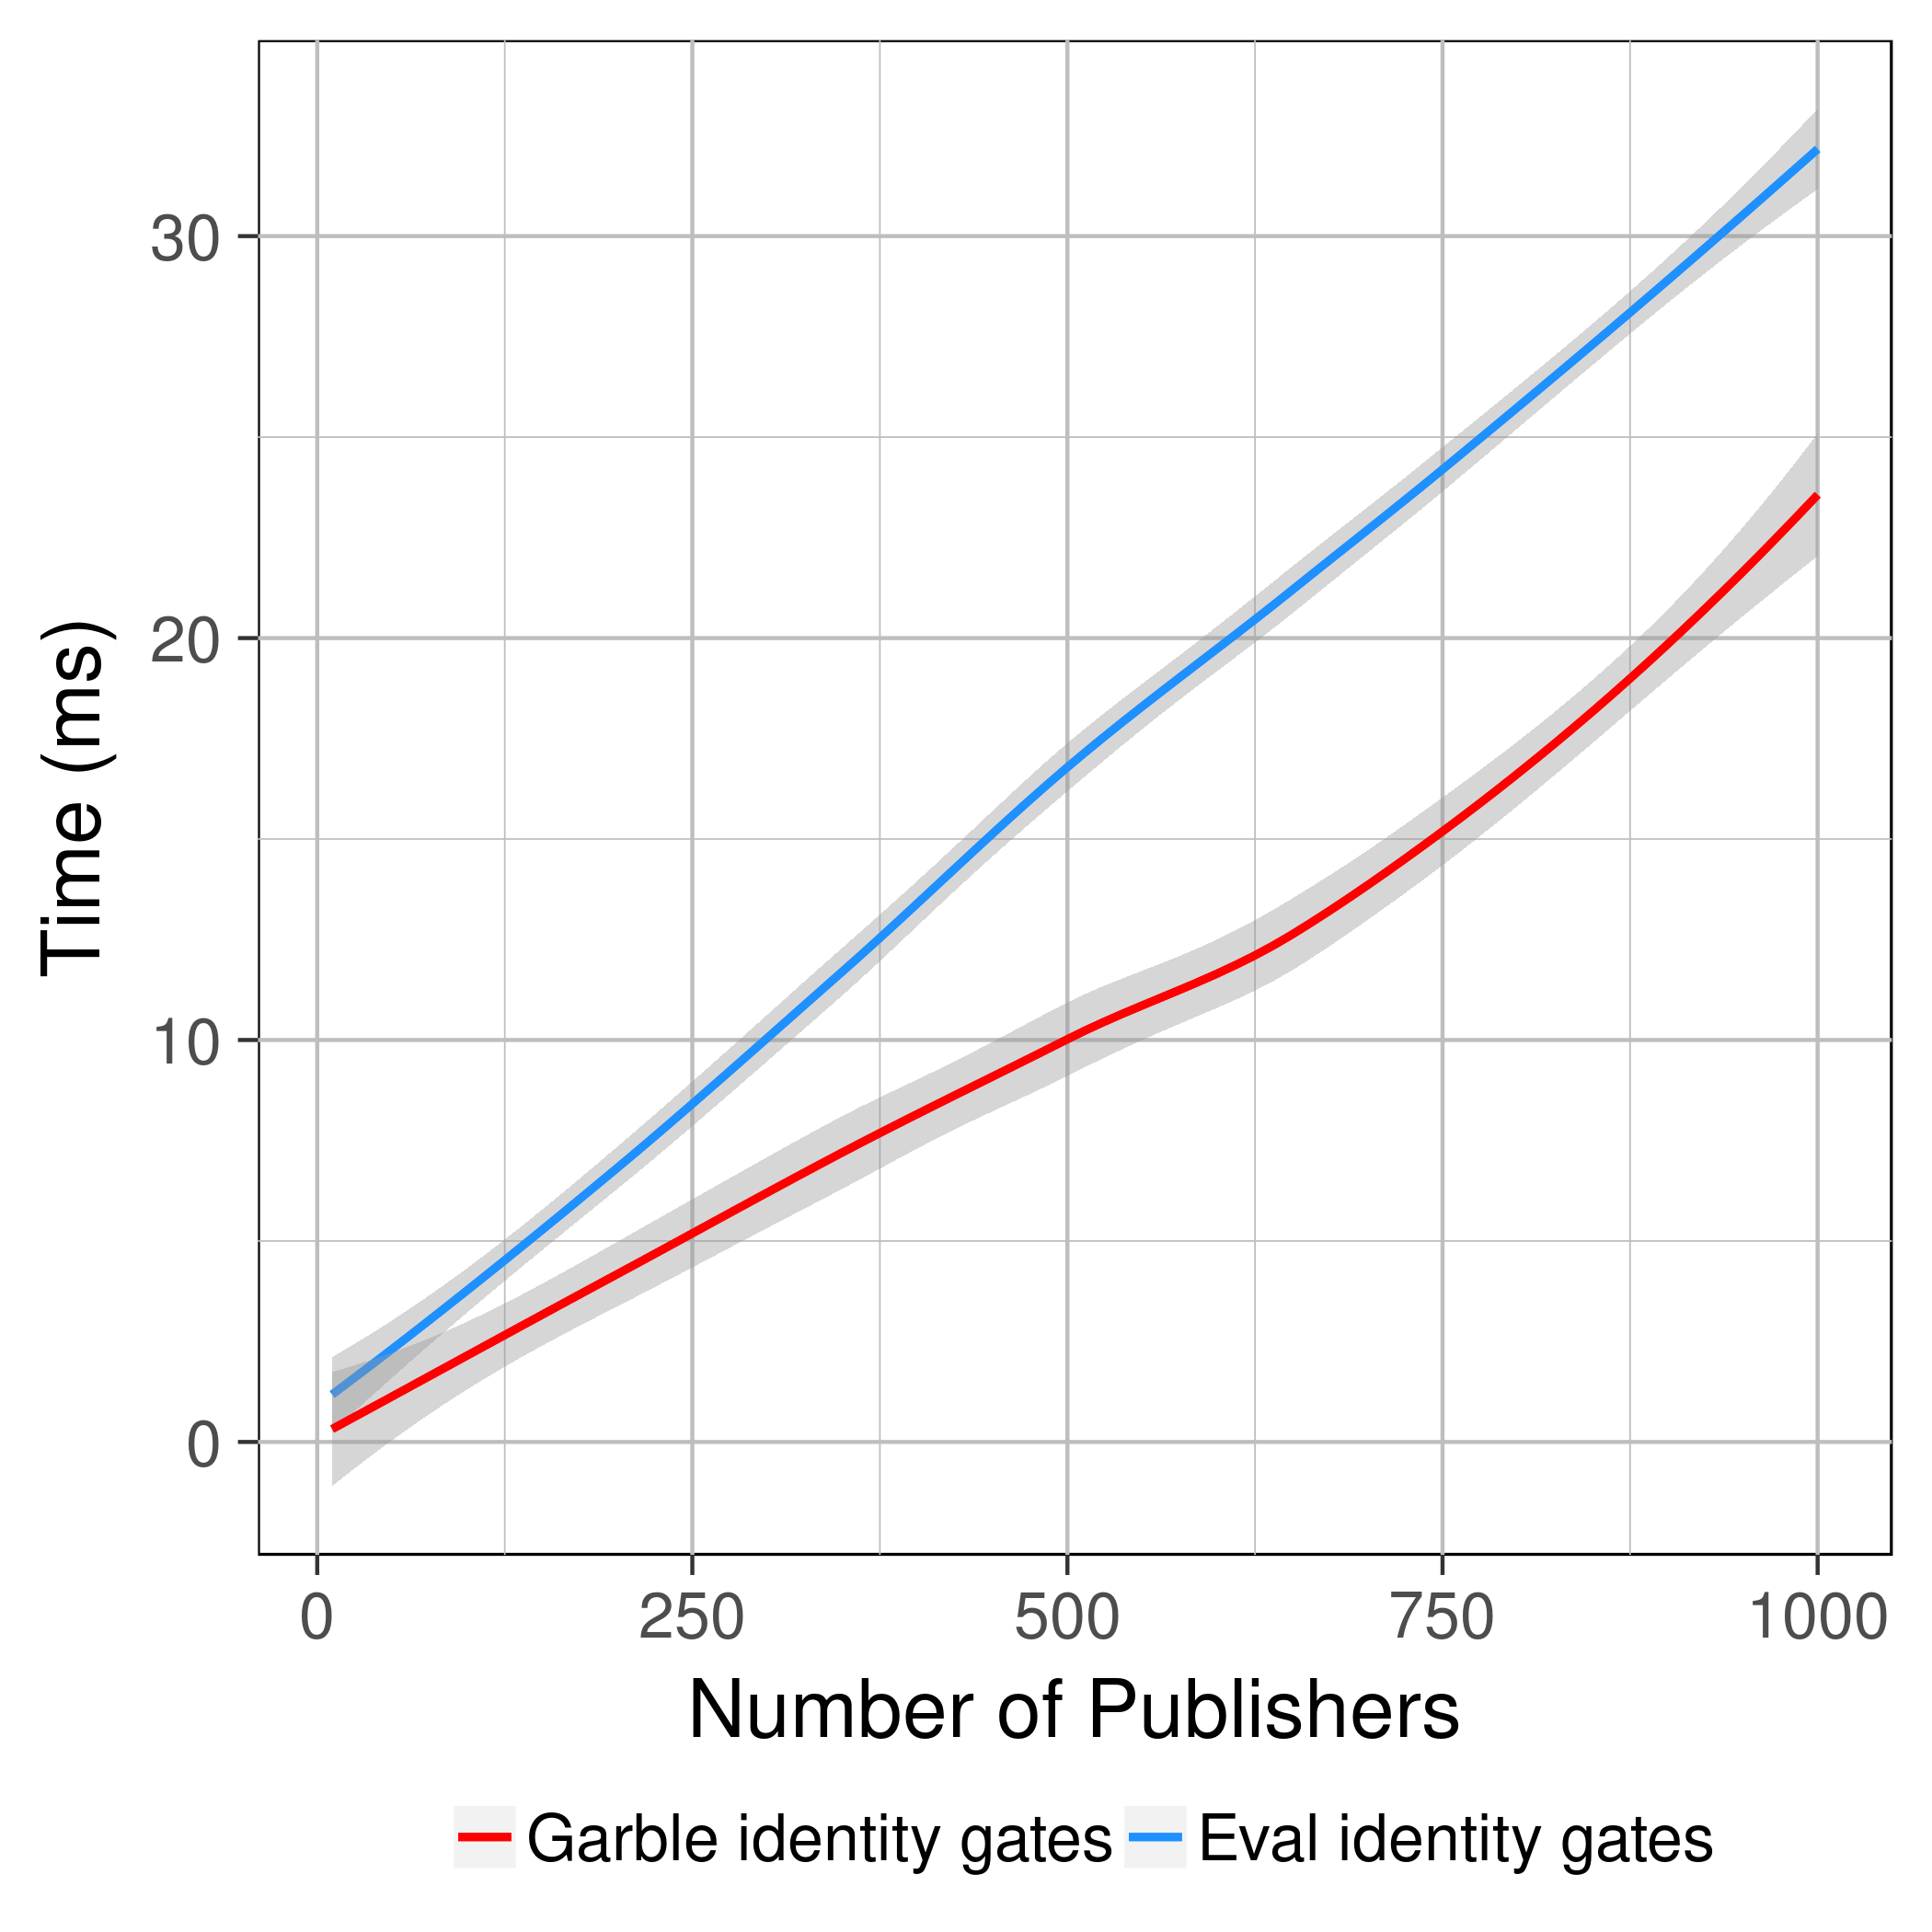
\includegraphics[width=0.32\textwidth]{plots/enc_dec.png}
  \caption{Time spent garbling and evaluating the identity input gates.
    Results obtained from the mean of all microbenchmark functions with 5
    repetitions each, with the confidence interval of 95\% shown in gray.}
  \label{micro-inputs}
\end{figure}

We can see in more detail a comparison of the time spent on garbling and
evaluating the identity gates in figure~\ref{micro-inputs}.  We expected the
garbling to be roughly twice the times of evaluating (garbling involves
encrypting two labels whereas evaluating involves decrypting one)

\begin{figure}
  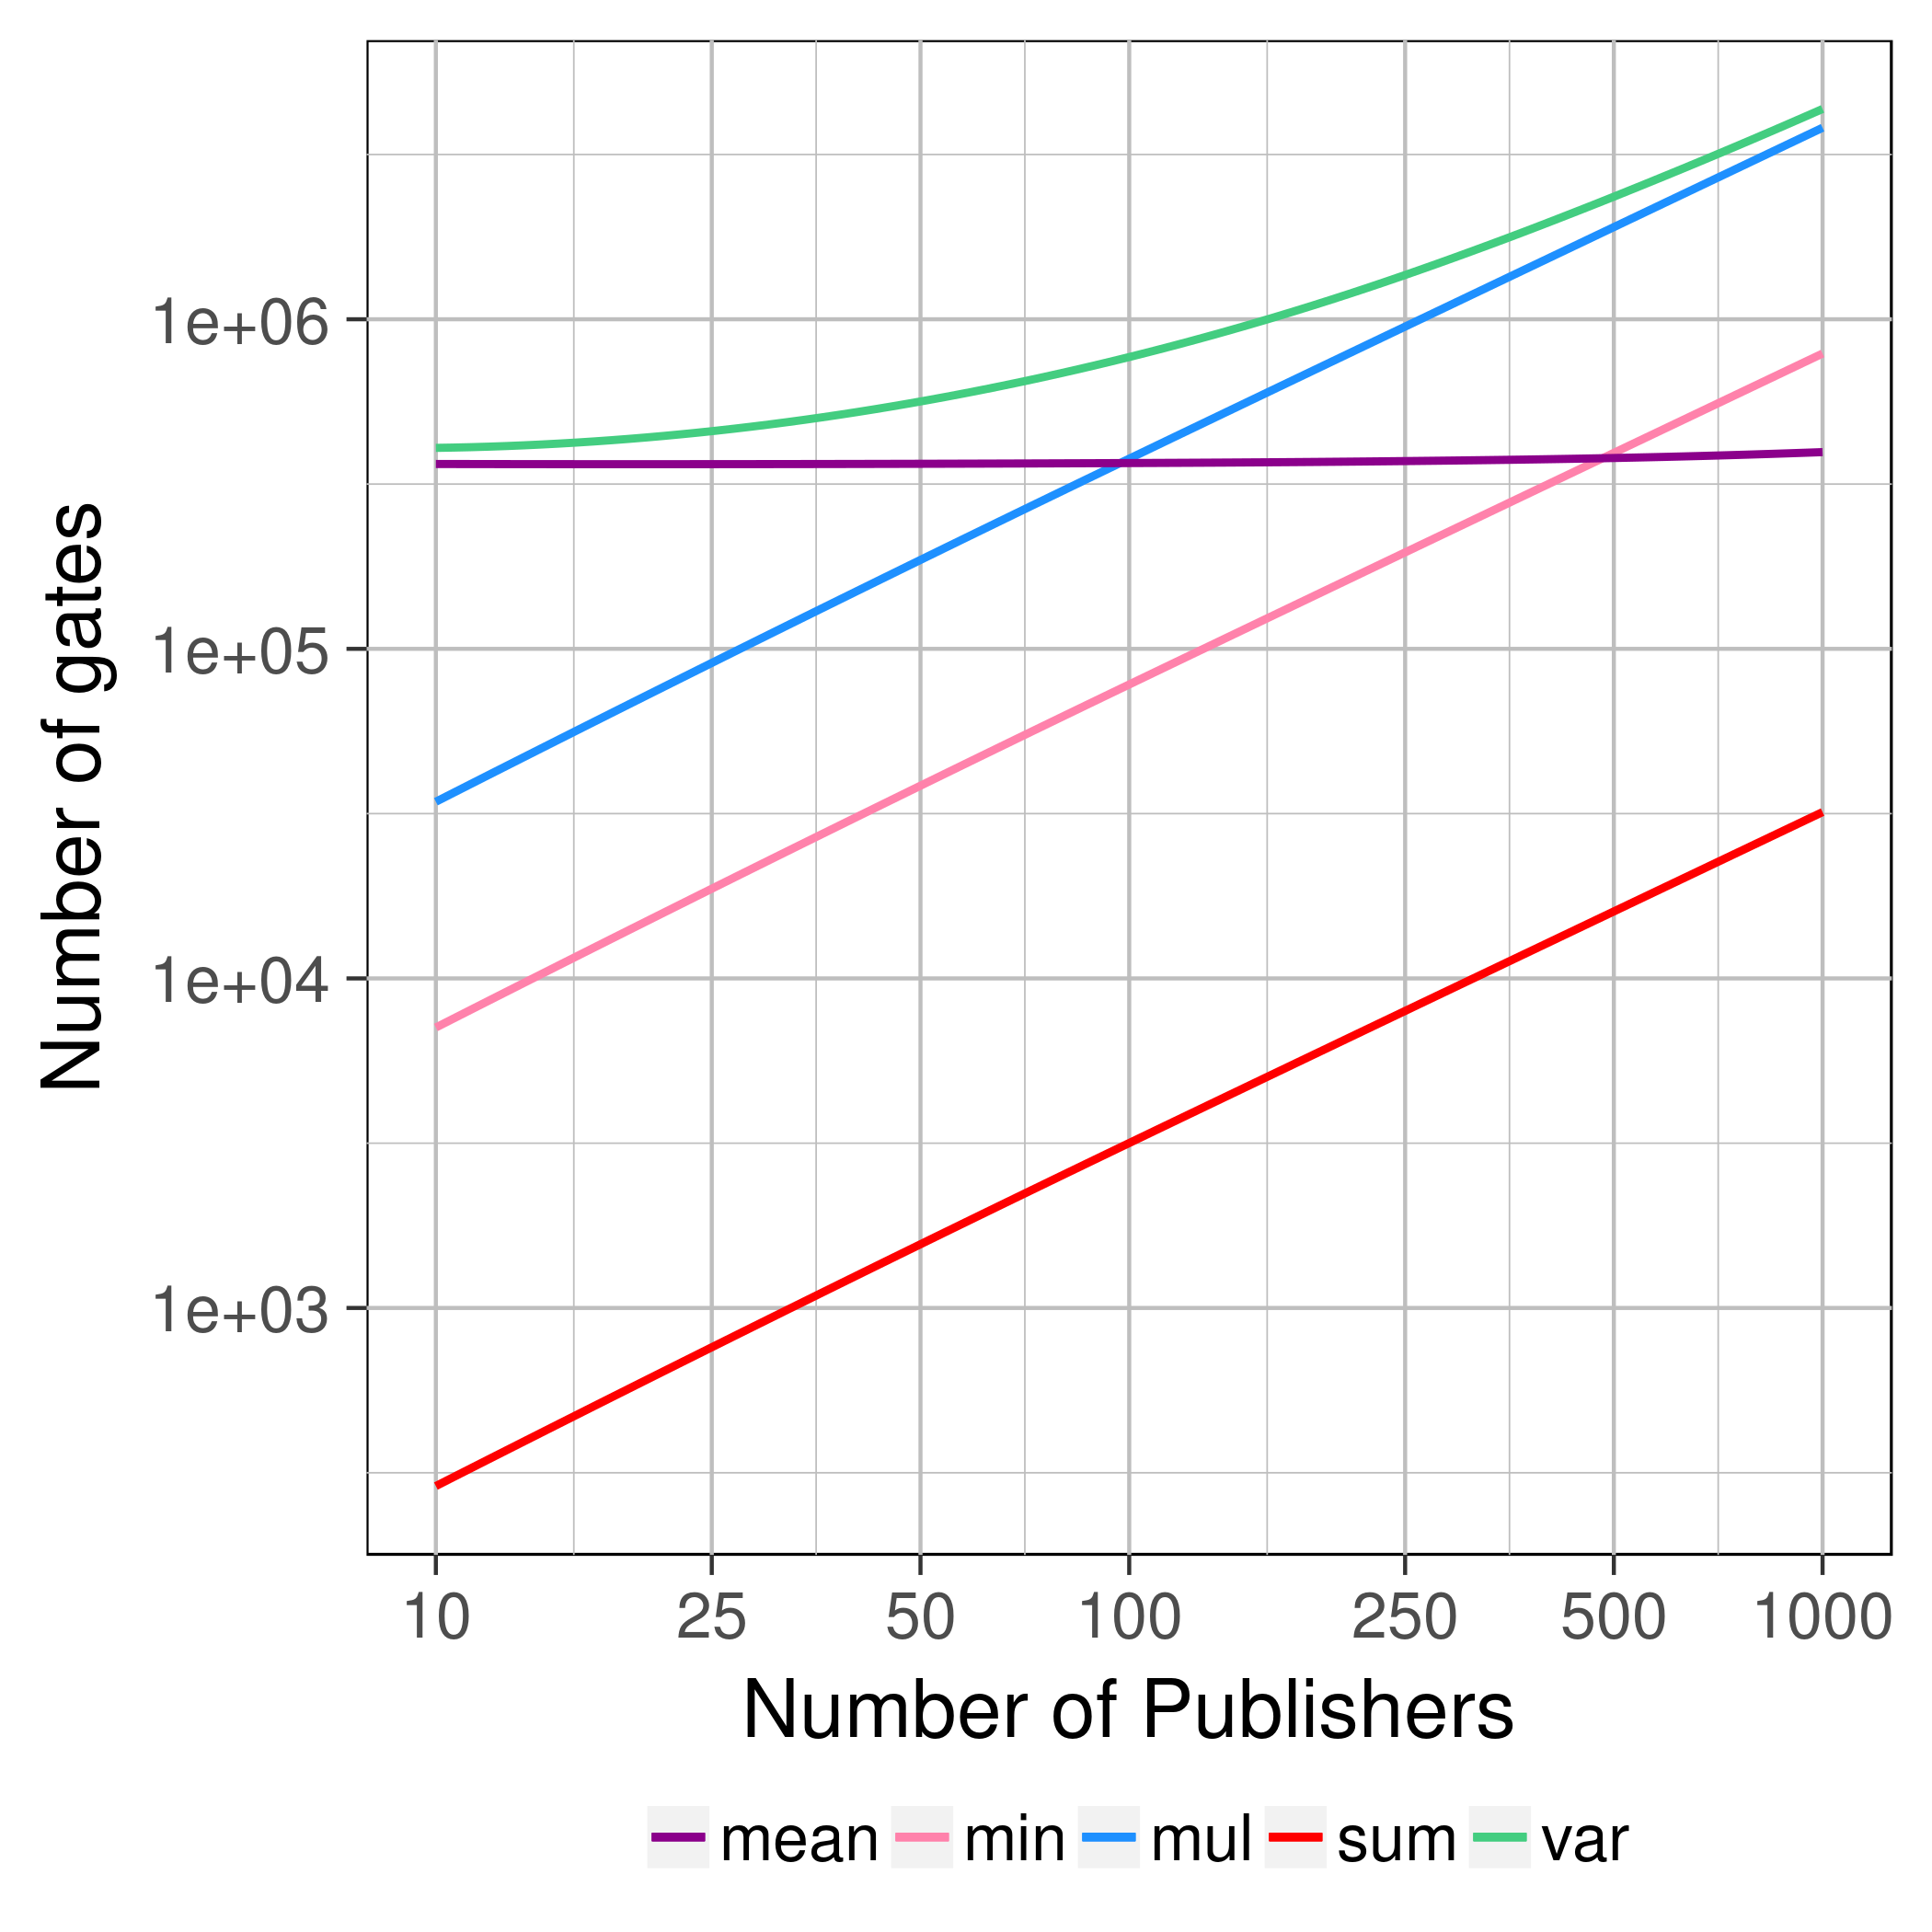
\includegraphics[width=0.32\textwidth]{plots/nonxor_gates_log.png}
  \caption{Non-XOR gates count per function used in the microbenchmarks.}
  \label{micro-nonxor}
\end{figure}

In figure~\ref{micro-nonxor} we show the number of non-XOR gates (that is, the
gates that incur a garbling and evaluating and that increase the size of the
garbled circuit) for every function.  We can clearly see the relation between
the number of the non-XOR gates and the cost of computing every function by
comparing shape of the plot with timing results shown in
figure~\ref{fig:micro-times}.

\begin{figure}
  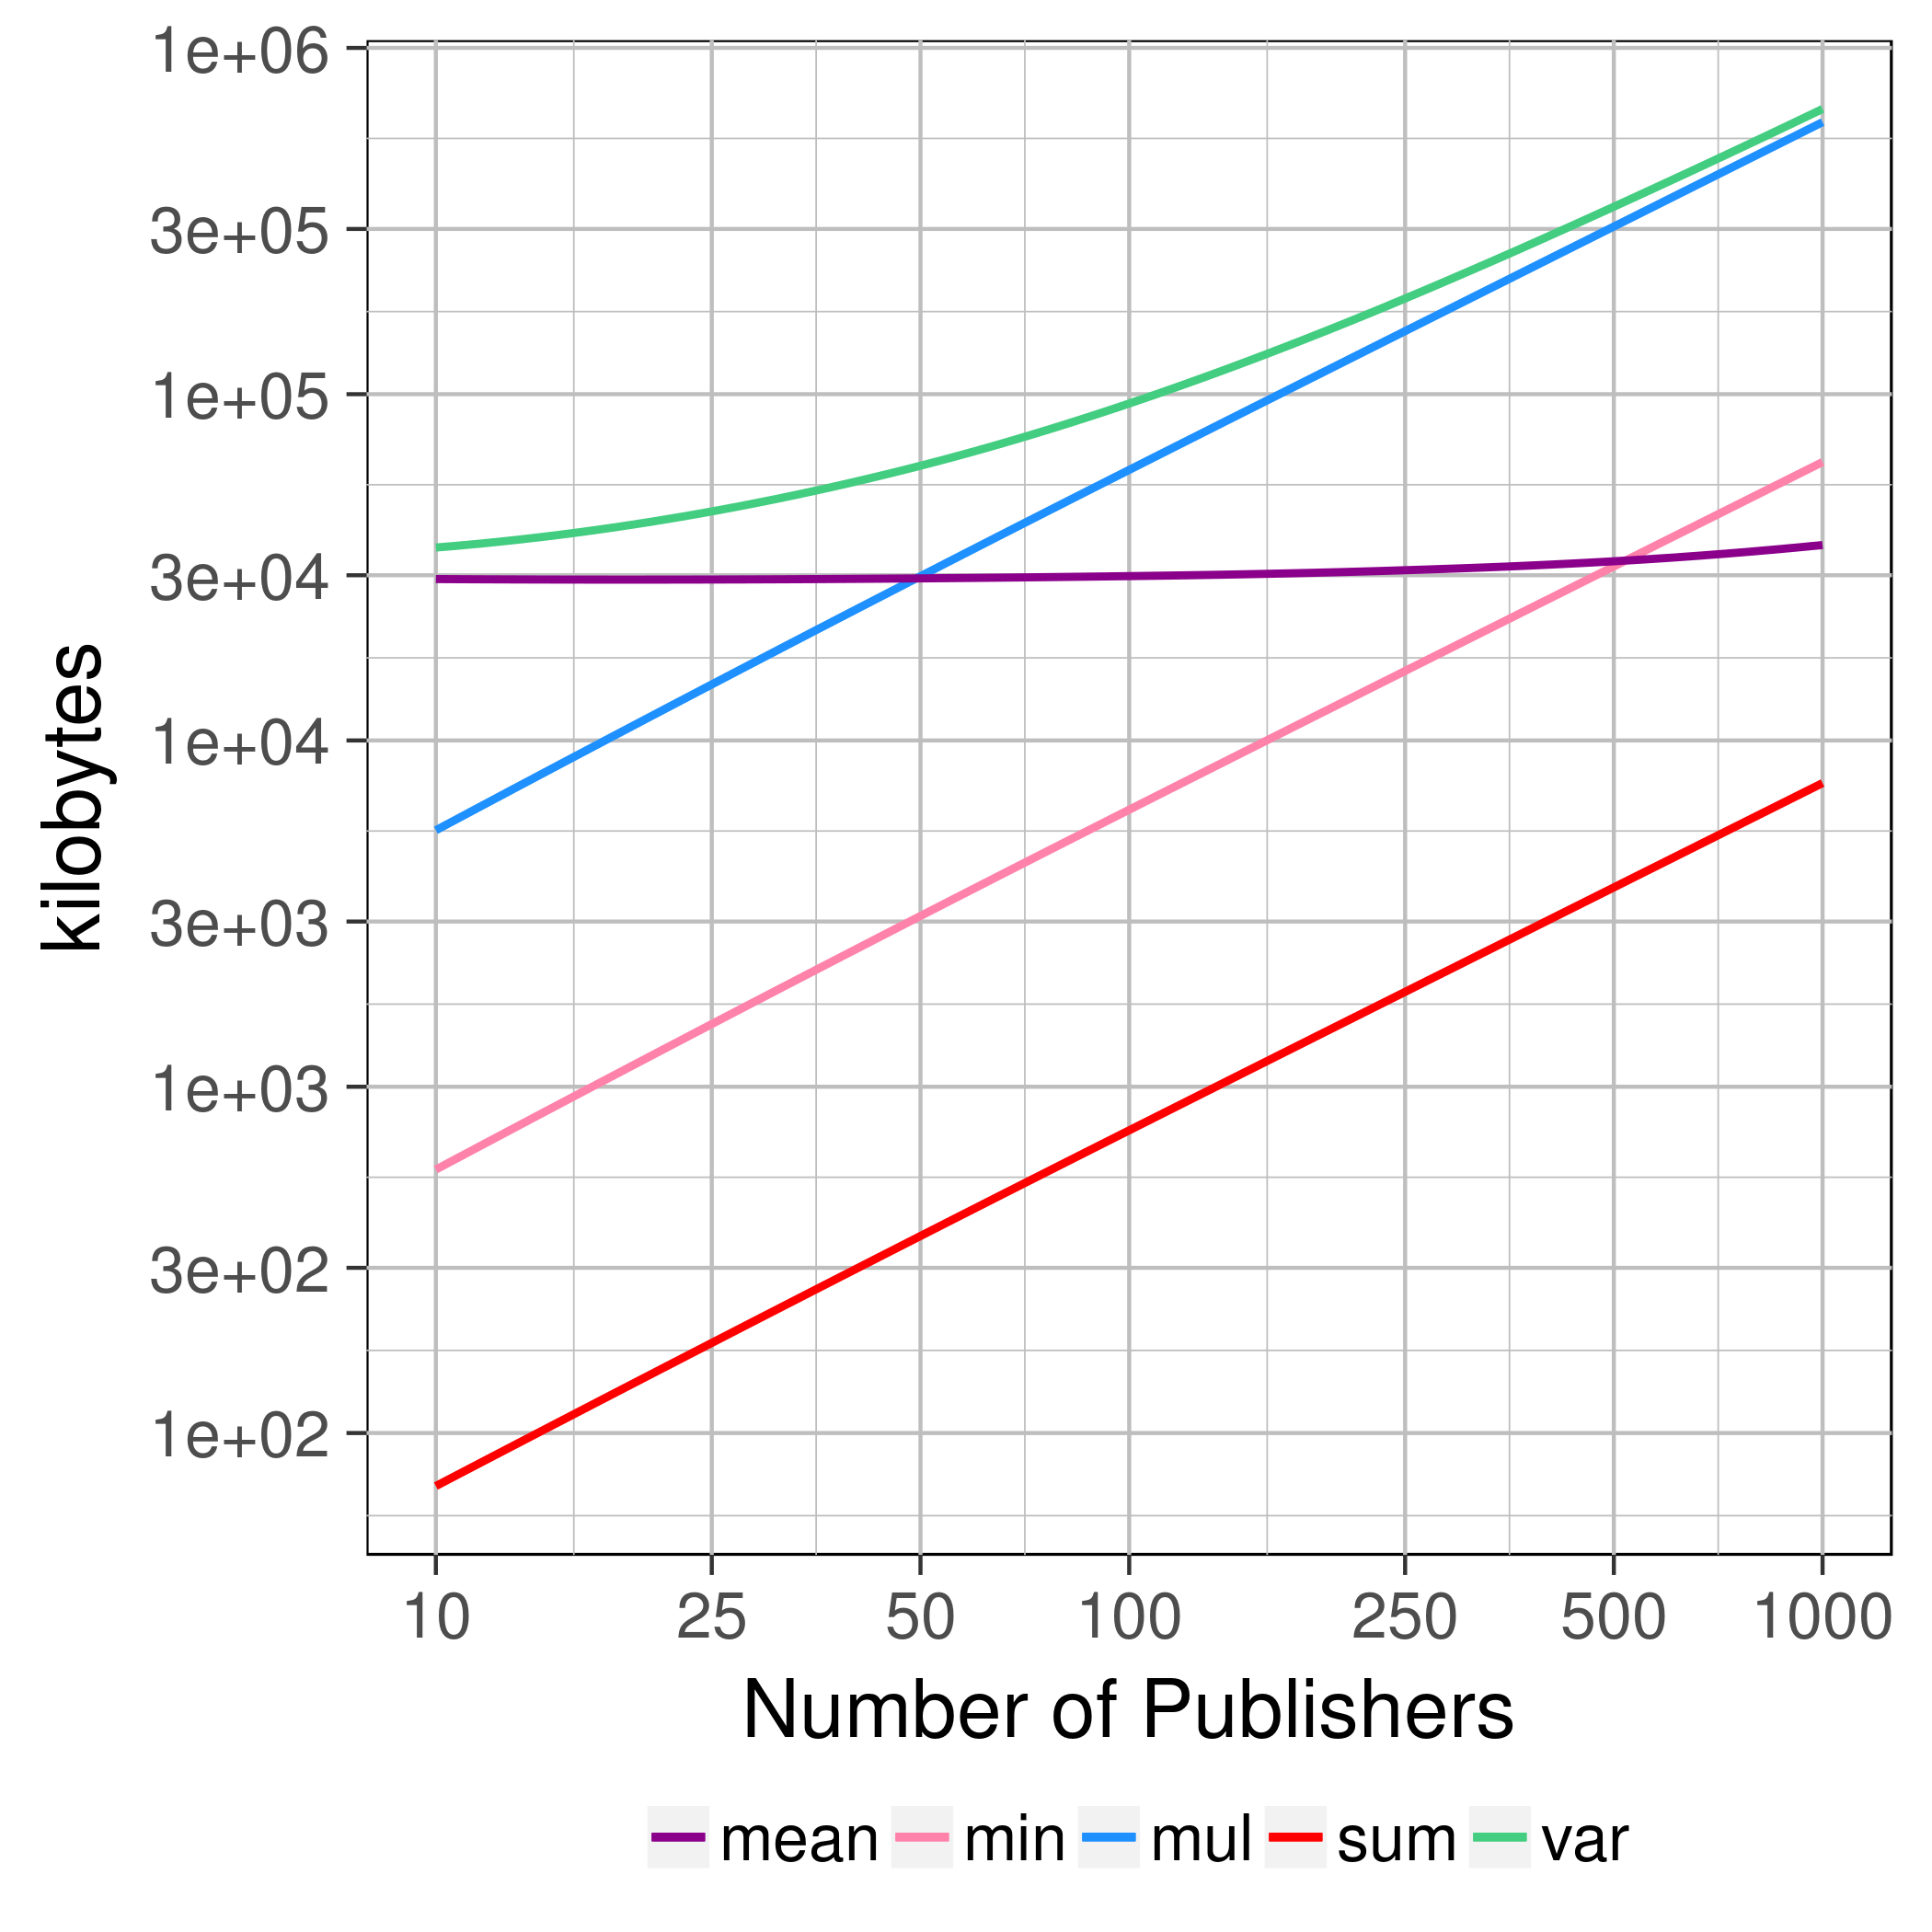
\includegraphics[width=0.32\textwidth]{plots/size_log.png}
  \caption{Size of the garbled circuit and the associated date required by the
    \broker to evaluate it.}
  \label{micro-sizes}
\end{figure}

In figure~\ref{micro-sizes} we see the transfer size between the \broker and
the \garbler for every function (that is, the size of the garbled circuit and
the associated data structures like the masking round used).  As expected, the
shape is very similar to the number of non-XOR gates for function shown in
figure~\ref{micro-nonxor}.  In the figure we can observe where the bottleneck
of using garbled circuits come from: the need to transfer such amount of data
over the network.  This fact makes the choice of network bandwidth between the
\broker and the \garbler critical, leading to very different results in
performance (which is dominated by the sending time) depending on the choice.
This figure also helps us understand the limits of using garbled circuits: the
\emph{variance} and \emph{multiplication} garbled circuits for 1000 Publishers
sizes are close to 700 MiB; considering the linear scaling we can easily
predict the point where the garbled circuits would be too big to fit into the
computer memory.

\begin{table}
    \begin{tabular}{l|*{4}{c}c}
      & \textbf{Sum} & \textbf{Mult} & \textbf{Mean} & \textbf{Var} & \textbf{Min/Max} \\
    \hline
    \textbf{Reduction} & 06.63 \% & 09.76 \% & 06.87 \% & 09.68 \% & 14.47 \% \\
    \end{tabular}
    \caption{Number of gates reduction for each microbenchmark function we
      would obtain by using the half-gates optimization.}
    \label{micro-and}
\end{table}

Considering the fact that we are not using the half-gates size optimization in
our garbled circuits, we show in table~\ref{micro-and} the reduction we would
observe for the experiments with 1000 Publishers if we had used such
optimization (computed by counting the number of AND gates used in each
circuit).  We observe the biggest reduction in the \emph{Min/Max} functions,
leading us to conclude that implementing the half-gates optimization would be a
clear improvement overall by reducing the sending time of the garbled circuits.

\vspace{-4pt}
\subsection{Applications}

We have prepared 3 concrete applications based on real IoT datasets to show
possible real usages of the presented protocol.

% Turonet, wireless propagation constant, linear regression
\smallskip
\noindent\textbf{Wireless propagation constant}

\noindent In this application we take the real time data provided by a testbed of IoT
nodes deployed in our university forming a mesh network.

The mesh network is formed by a fixed number of nodes deployed in different
static locations in the same building that connect to each other via wireless.
Every node tries to connect to the others unless they are too far, giving us an
upper bound of $n \cdot (n-1)$ connections where $n$ is the number of nodes.
Each node periodically publishes the received signal strength ($RSS$) in dBm of
the nodes it is connected to; and this measure can fluctuate over time due to
fading.

We are interested in estimating the wireless propagation constant ($\eta$) in
the medium while preserving the privacy of the nodes (that is, their location,
the distance between nodes and their reported signal strength measures).
The value of $\eta$ can be useful in characterizing the radio propagation
environment and performance of the network and it can be derived from the
following formula: \mbox{$RSS = -10 \cdot \eta \cdot log_{10}(distance) - C$}.
We will estimate $\eta$ by finding a linear model for the $RSS$-distances pairs
obtained from the nodes.

% This was my original interpretation.  Since we already have the experiments,
% let's move this to the Environmental Berkeley indoor sensing data, but leave
% the formula description and linear regression explanation here.
In particular, we perform a linear regression so that we can model the $RSS$ as
a linear combination of a logarithmic function of the distance.  To estimate
the parameters of the one dimensional linear model ($y = ax + b$) we use the
ordinary least squares technique, which gives us the following closed-form
formula:

\[
\begin{pmatrix} b \\ c \end{pmatrix} =
\left( \sum_{i=1}^n \begin{pmatrix} 1 \\ x_i \end{pmatrix}
  \begin{pmatrix} 1 & x_i\end{pmatrix}\right)^{-1}
\left( \sum_{i=1}^n y_i \begin{pmatrix} 1 \\ x_i \end{pmatrix}\right)
\]

Evaluating the formula requires an inversion of a $2 x 2$ matrix, which we perform
by following the analytic solution.

For the evaluation of this application we construct a virtual scenario which
simulates the IoT nodes by running one Publisher per node in a separate
computer.  The Publishers will publish the $log_{10}$ of the distances to their
peers as an initial step, allowing the \broker to store these values for some
time avoiding the constant retransmission of these constants.  After this, the
Publishers will be sending values at the same rate of the nodes in order to
obtain the same performance results we would get by using live data from the
actual testbed.  Following our protocol, we will be estimating the wireless
propagation constant periodically, using the values received form the
Publishers.  We will vary the number of Publishers to analyze how this
application scales (notice that the number of inputs for the linear regression
formula grows quadratically when the number of nodes increases linearly)

\begin{figure}
  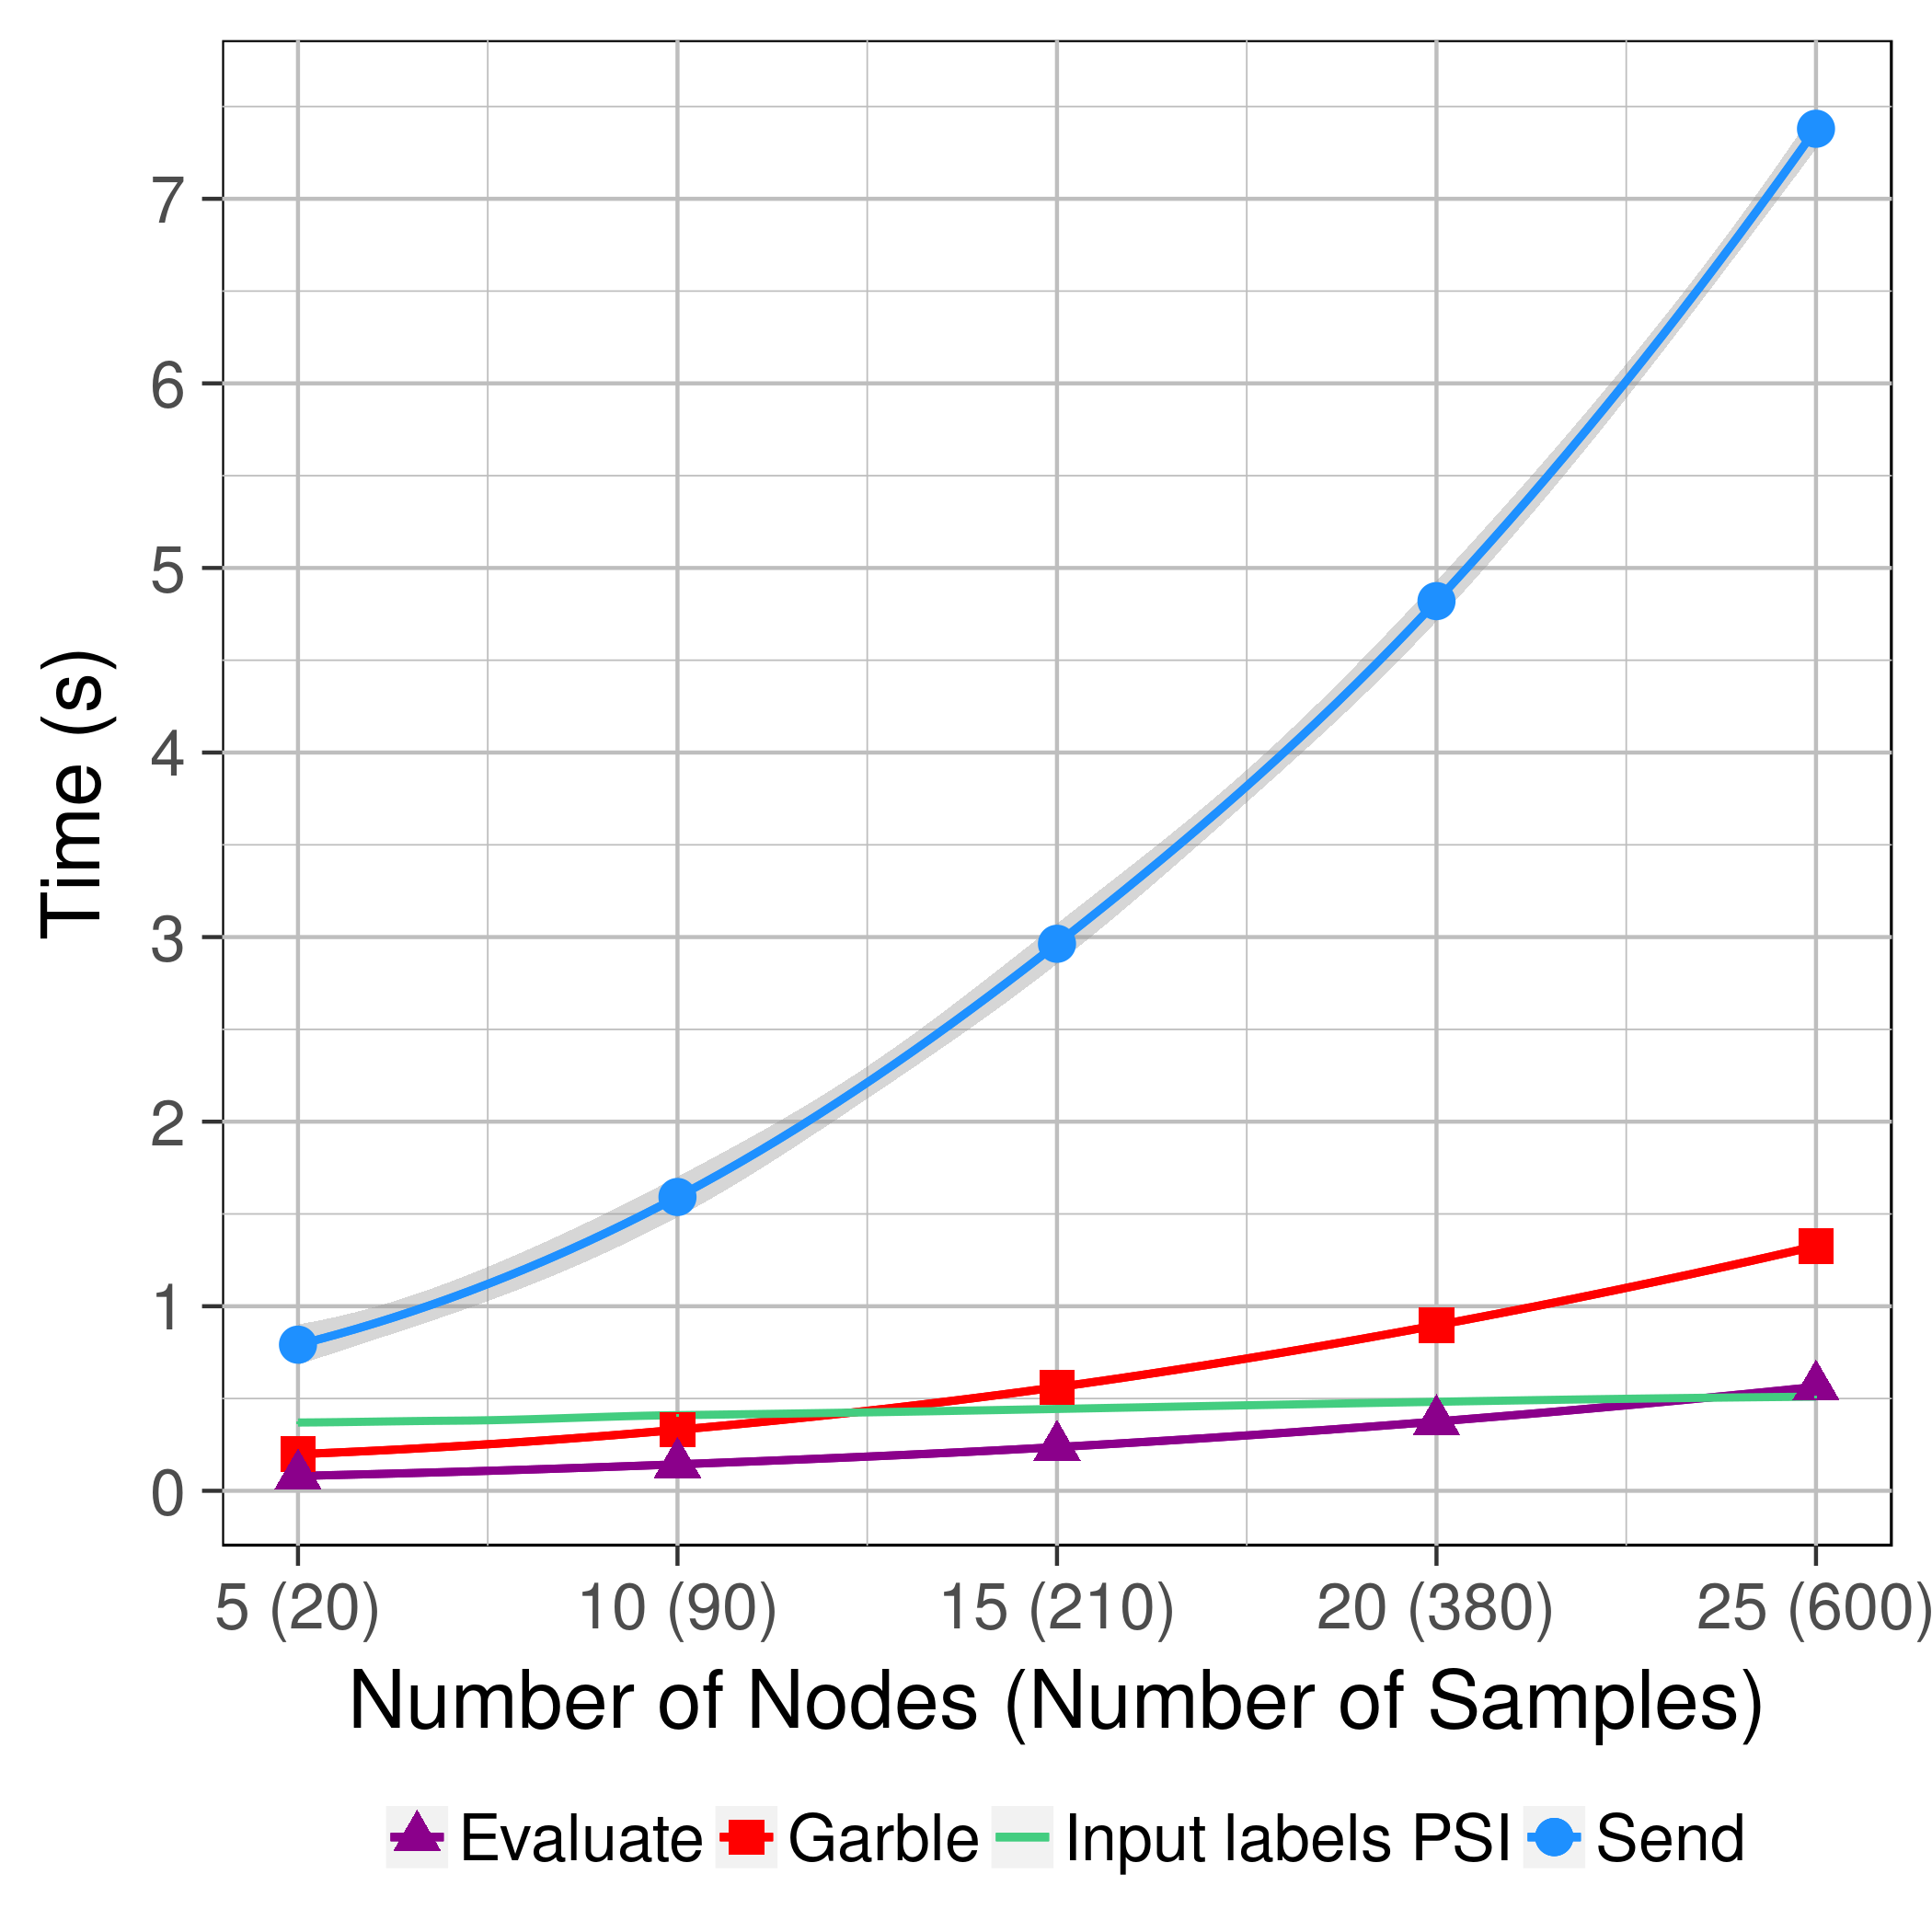
\includegraphics[width=0.32\textwidth]{plots/turonet.png}
  \caption{Mean time required for garbling, evaluating and sending the garbled
    circuit to the \broker for a varying number of nodes in the \emph{wireless
    propagation constant} application.  Results obtained from the mean of 5
    repetitions for each configuration, with the confidence interval of 95\% shown
    in gray.}
  \label{turonet-times}
\end{figure}

We show the results of the evaluation in figure~\ref{turonet-times}, where we
can clearly see that the cost for this application quickly grows with the
number of nodes.  Our experiments end at 25 nodes because at at 30 Nodes we
would be dealing with $30 \cdot 29 = 870$ samples to perform the correlation,
which corresponds to a garbled circuit of size bigger than 1 GiB.  At this
magnitude we hit a limit on the encoding used when marshaling the garbled
circuit in the Go RPC implementation, which doesn't support data structures
bigger than 1 GiB.  Notice however that we are using all the samples to
calculate the linear regression even though a random sample of a smaller size
would suffice; and that our scenario considers that all nodes are
interconnected, which will usually not be the case when the number of nodes
reaches a significant value.

% Environmental Berkeley indoor sensing data, correlation
\smallskip
\noindent\textbf{Correlation of environmental indoor sensing data}

\noindent For this application we will be using the environmental indoor sensing data
provided by the Intel Berkeley Research
lab~\cite{berdata}.  This dataset provides 2.3 million readings collected
from sensors with the following values: temperature in degree Celcius, humidity
in percentage and light measured in Lux.

We are interested in finding relationships between pairs of data streams, each
coming from a different sensor, while maintaining the individual readings
private.

In this application's scenario, we assume that each sensor would be an
individual Publisher that sends readings periodically.  The \broker would
accumulates streams of published values from each sensor, and when requested,
the it would samples pairs of those streams at random over a specific period of
time to perform a correlation analysis between the two.  For our experiments we
vary the number of samples and simulate the application by supplying the \broker
with the given number of samples in a batch.

% Formula:
The correlation is a measure of statistical relationship among pairs of
variables in which higher value represents higher dependence.  Following the
Pearson's product-moment coefficient, we can measure the dependence between
samples of two variables (in our case, sensor readings) using the following
closed-form formula:

\vspace{-8pt}
\[
r_{xy} = \frac{\sum_{i=1}^n (x_i - \bar{x}) (y_i - \bar{y})}
{\sqrt{\sum_{i=1}^n (x_i - \bar{x})^2 (y_i - \bar{y})^2}}
\]

To improve efficiency, we evaluate the squared correlation ($r_{xy}^2$) to avoid
computing the square root in the function circuit, which would be an expensive
operation.

As a comparison, we will also evaluate the cost of computing the
one-dimensional linear regression over two streams of values with a varying
number of samples, which also gives us information about the relationship
between the two data streams.

\begin{figure}
  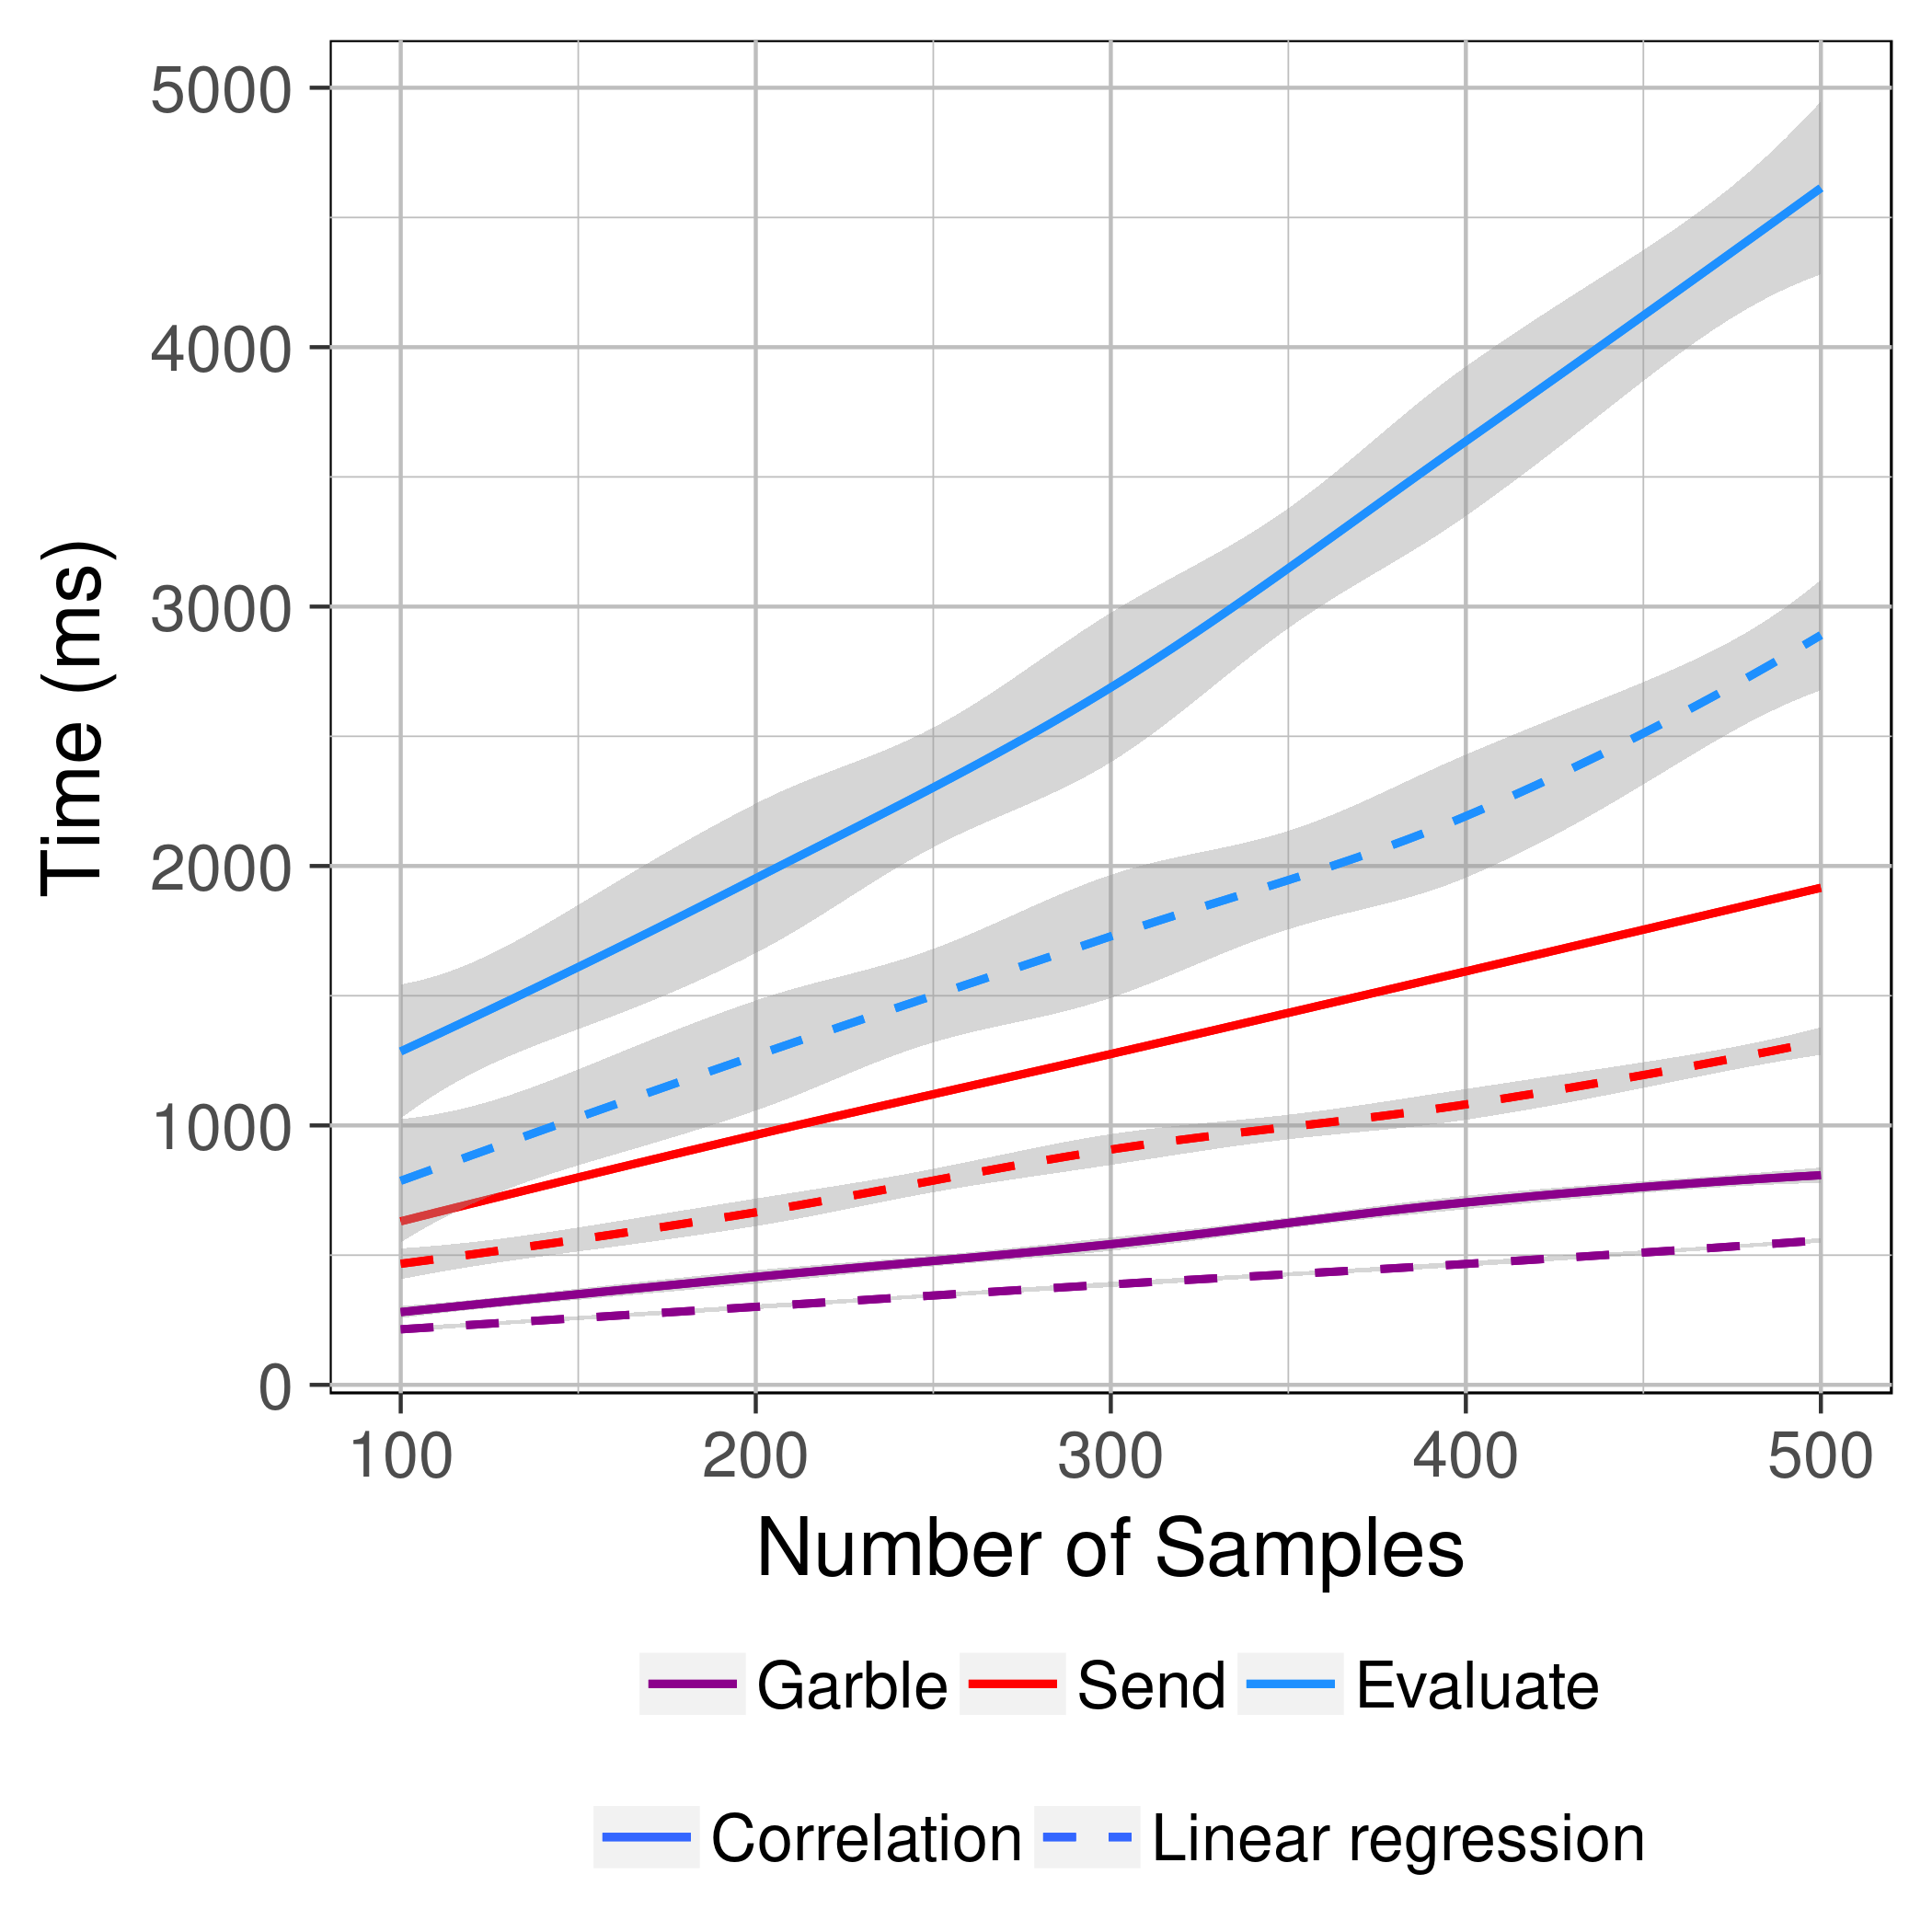
\includegraphics[width=0.32\textwidth]{plots/stream.png}
  \caption{Mean time required for garbling, evaluating and sending the garbled
    circuit to the \broker for computing the squared correlation and linear
    regression of data streams.  Garbling and evaluating includes the time to
    garble and evaluate the input identity.  Results obtained from the mean of
    5 repetitions for each configuration, with the confidence interval of 95\%
    shown in gray.}
  \label{stream-times}
\end{figure}

As we can see in figure~\ref{stream-times} the cost of computing the
correlation is roughly the double of the cost of computing the linear
regression.  Taking this result into consideration, we could devise a more
efficient statistical relationship measure: for instance, we could first
compute the linear regression and then find a normalized error between the
linear model and the samples.

% LAX parking lot dataset, statistics
\smallskip
\noindent\textbf{Daily statistics of airport parking lots}

\noindent The dataset for this application is the live status of the parking
lots of a major airport~\cite{LAX}.  In particular, the airport provides
updates of the number of occupied and free parking spaces for each one of the 9
parking lots every 5 minutes.  This makes a total of 288 published values per
day per parking lot.

In such application we would be interested in obtaining daily statistics of the
parking lots without revealing data at fine time granularity.  We will only
allow obtaining data accumulated throughout the day while preserving the
privacy of the individual parking lots values.

For this scenario, we will have 9 Publishers, one for each lot, which will be
sending the current number of free and occupied spots every 5 minutes.  We
simulate the Publishers by running them together in a single computer.  The
\broker will accumulate the data from each day and compute the daily statistics.

Using the occupied spots data, we will provide the \emph{mean}, \emph{min/max},
and \emph{variance} of the number of cars in all the lots combined during a
day.  Using the free spots data, we will compute which lot had more free spots
and which one had less free spots on average during the day.  We will refer to
this later result as the \emph{rank}.

\begin{table}
    \begin{tabular}{l*{3}{r}r}
    \textbf{Statistic}  & \textbf{Garble} & \textbf{Send} & \textbf{Evaluate} & \textbf{Size} \\
    \hline
    Mean       & 199.8 ms & 461.7 ms & 98.7  ms & 45.0 MB \\
    Max/Min    & 163.3 ms & 345.2 ms & 84.9  ms & 32.3 MB \\
    Variance   & 500.7 ms & 2376.3 ms & 236.1 ms & 222.4 MB \\
    \hline
    Rank free  & 121.3 ms & 181.0 ms & 67.5 ms & 17.0 MB \\
    \end{tabular}
    \caption{Mean time required for the different steps of the protocol to
      evaluate different statistical measures of the parking lot dataset.
      Garbling and evaluating includes the time to garble and evaluate the
      input identity.  The mean time required to perform the Private
      Intersection Set of the input labls in all cases has been 
      \mbox{$1107.4 \text{ } ms$}.  Results obtained from the mean of 5 repetitions for
      each configuration.}
    \label{stats-times}
\end{table}

We can see the results of the evaluation in table~\ref{stats-times}.  We
observe that for the given amount of daily data, the statistics can be computed
in a short period of time; the \broker and \garbler could be computing daily
statistics from data coming from many more sources.  The most expensive
operation is the \emph{variance}, which coincides with the results obtained
from the microbenchmarks; and the cheapest one is the \emph{rank}.

% SKIP: 3. Road Volume sensor traffic, evaluation of the expected time to follow a path
%\paragraph{Estimation of time required to follow a path with traffic}
% http://rtmap.metro.net/ <- Not working (2017-05-15).

% SKIP: 5. Smart bill, monthly electricity bill with different cost per hour of the day / threshold.

% TODO: Discussion: bottlenecks.

\vspace{-4pt}
\subsection{Discussion}

\noindent\textbf{Bottlenecks.}  As expected, the time spent sending the garbled
circuit from the \garbler to the \broker is the most expensive part of the
protocol, and thus is the current bottleneck.  This means that the quality and
bandwidth of the network connection between the \broker and the \garbler is of
critical importance.

The actual fraction (without considering the \PSI) of time spent on sending the
garbled circuit varies depending on the circuit function and the number of
Publishers, ranging from about 50 \% as in the rank calculated in the
\emph{daily statistics of airport parking lot} to about 80\% as in the
\emph{wireless propagation constant} application with 25 nodes.

When we consider the results of the \PSI simulation, we observe that for the
most lightweight applications it requires more time than all the garbled
operations combined, whereas in the most heavyweight applications it can become
as small as the 10\%.

The total time required for computing the functions securely in our different
applications experiments range from about two seconds as in the \emph{daily
statistics of airport parking lot} to a about 14 seconds as in the
\emph{correlation of environmental data} with 500 samples.  Considering the
fraction of time spent sending the garbled circuit in the more costly
application configurations, we could get a good estimate of the total time by
just knowing the number of non-XOR gates used (which would determine the size
of the garbled circuit) and the network bandwidth available from \broker to
\garbler.

The results obtained are perfectly suitable for computing several functions
like the ones presented in the applications in a \broker-\garbler pair
periodically.  For example, 6 different applications similar to the ones shown
could be running every minute.  In our experiments, all the garbling and
evaluating steps have been computed in serial in order to get result measures
with the minimum fluctuation, but in a real system, several functions could be
run at the same time allowing for concurrent garbling and evaluation making use
of all the CPU cores available.

\noindent\textbf{Optimizations.} In general, the second most expensive part of
the protocol is running the \PSI.  Decreasing the required time for this
operation would have a significant decrease on the cost of our lightweight
applications.  We could take advantage of the fact that in our \PSI setting,
one of the parties (the \garbler) has the full set, and the other one (the
\broker) a subset of it.  Another possibility would be to try different ways of
batching the labels in the \PSI.

The garbling and evaluation of the identity gates could be optimized by
incorporating the operations in the C code of libgarble.  Even though the
Go implementation of the AES encryption and decryption functions use the
Intel AES-NI hardware instructions, conversions from byte vectors to AES blocks
and vice versa slow down the operation.  On the other hand, libgarble works
natively with 128 bits data types (the size of an AES block) by using the Intel
SSE2 extensions, thus not requiring any conversion during
encryption/decryption.


\section{Conclusion}
\label{sec:conclusion}

We propose a secure publish-process-subscribe protocol and built a full-fledged
system with several new system contributions. Our system uses \MQTT protocol to
offer a lightweight protocol for publishers and subscribers.

Our system evaluation shows that our system is practical, efficient, and
scalable to run both basic arithmetic functions, such as, summation, minimum,
and variance; as well as more complex functions, such as, correlation and
linear regression, on a significant number of inputs. In particular, our system
is able to compute the one-dimensional linear regression of $600$ samples in
$10.5$ seconds. It can also compute $4$ basic statistical parameters (mean,
max/min, variance) on the daily accumulated data from streams publishing at $5$
minutes interval in less than $7$ seconds.

The most expensive part of our protocol is sending the garbled circuit, usually
more than half of the overall cost in garbled circuits.  The second most
expensive part is running the private-set-intersection protocol required to
detect malicious Publishers; which we believe could be improved in the future.


 % TODO: replace with your brilliant paper!

%\appendix
%Note that in the new ACM style, the Appendices come before the References.

\begin{acks}
% TODO: For the submission, don't include acknowledgments since they would most
	% likely deanonymize you.
\end{acks}

\bibliographystyle{ACM-Reference-Format}
\bibliography{refs,bkpps}

\end{document}
